%module geschreven door Jeroen Dehaene zomer 2008

% geen wijzigingen in 2011 /2012 (behalve datum en include->input voor nieuwe miktex)/ Riet Callens

%2018 Riet: omgezet naar pdf-te
%macro's voor zomercursus wiskunde - Groep Wetenschap & Technologie - 29 januari 2008
%Bart Bories en Riet Callens
%aangepast door Riet Callens op 23/06/2009
%aangepast door Riet Callens op 9/7/2009 (newtheorem oefening toegevoegd)
%aangepast door Riet Callens op 27/07/2012 voor pdf-tex
%aangepast door Riet Callens op 22/08/2012 voor vragen ijkingstoets (numopl}
%aangepast door Riet Callens op 1/08/2019 voor implementatie QR-codes - qrslidesA,qrslidesB,qrclip,qrapplet


\documentclass[a4paper,12pt,twoside]{ximera}
\usepackage{qrcode}
\usepackage{etex}
%standaard pakketten
%\usepackage{a4wide}
\usepackage[dutch]{babel}
\usepackage{hyphenat}
\usepackage{xcolor}
\definecolor{KULblauw}{RGB}{26,67,121}
%\usepackage[color=white,linkbordercolor=white ]{hyperref}
\usepackage{amsmath}
\usepackage{amssymb}
\usepackage{amsfonts}
\usepackage{graphicx}
\usepackage{wrapfig}
%\usepackage{pst-plot}
%\usepackage{pst-pdf}
%\usepackage{enumerate}
\usepackage{tikz}
\usepackage{pgfplots}
\usetikzlibrary{through,calc,intersections}
\pgfplotsset{axis lines = center}
\pgfplotsset{axis equal image}
\pgfplotsset{xlabel = x}
\pgfplotsset{ylabel = y}
\pgfplotsset{xlabel style={below right}}
\pgfplotsset{ylabel style={above left}}

%\usepackage{color}
%\usepackage[thmmarks,framed,amsmath]{ntheorem}
\usepackage{answers}

%definities nieuwe omgevingen
\Newassociation{opl}{Oplossing}{ans}
\Newassociation{numopl}{NumOplossing}{numans}
%\theoremstyle{break}
%\theoremheaderfont{\normalfont\bfseries}
%\theoremsymbol{}

%\theorembodyfont{\upshape}
\newtheorem{oefening}{Oefening}[section]
\newtheorem{oefening2}{Oefening}
\newtheorem{soefening}{Samengestelde oefening}
\newtheorem{vraag}[oefening2] {Vraag}
\newtheorem{oefeningen}[oefening]{Oefeningen}
\newtheorem{taak}{Taak}
\newtheorem{definitie}{Definitie}[section]
\newtheorem{voorbeeld}[definitie]{Voorbeeld}

%nieuwe commando's
\newcommand{\qrslidesA}[1]{Lesmateriaal gebruikt in het A-programma: \vspace{3mm}\\  \qrcode{#1} \href{#1}{\tiny{#1}}\\\vspace{3mm}}
\newcommand{\qrslidesB}[1]{Lesmateriaal gebruikt in het B-programma: \vspace{3mm}\\  \qrcode{#1} \href{#1}{\tiny{#1}}\\\vspace{3mm}}
\newcommand{\qrclip}[1]{\qrcode{#1} clip: \href{#1}{\tiny{#1}}}
\newcommand{\qrapplet}[1]{\qrcode{#1} applet: \href{#1}{\tiny{#1}}}

%bladschikking
\voffset=-1in
\topmargin=1.5 cm
\headheight=2cm
\headsep=1cm
\textheight=22cm
\footskip=1.2cm
\hoffset=-1in
\oddsidemargin=2.5cm
\evensidemargin=2.5cm
\textwidth=15.5cm
\marginparsep=0cm
\marginparwidth=0cm
\setlength{\parindent}{0pt}
\setlength{\parskip}{5 pt}

\newcounter{module}



%hoofding +kop- en voettekst
\usepackage{fancyhdr}
\pagestyle{fancy}
\renewcommand{\sectionmark}[1]{\markboth{\small{\textsc{\thesection.\ #1}}}{}}
\def\hoofding #1#2#3{\newpage
							\thispagestyle{empty}

             \hrule
             \begin{center}
             {\large {\textsc{Zomercursus Wiskunde}}}

             \bigskip
%             \begin{minipage}[c]{2cm}\includegraphics[width=2cm]{./../macros/sedes.jpg}\end{minipage}

             \bigskip
             {\textsc{KU Leuven}}\\
						 {\textsc{Groep Wetenschap \& Technologie}}
						
						 \bigskip
             {\textsc{September 2019} }
             \bigskip

             {\large \textsc {Module \arabic{module}\\ \bigskip #1}} \\
             (\small{versie \today})
             \bigskip

             \end{center}

             \hrule

             \bigskip
#2

\bigskip

#3

             
						 \newpage
						 \lfoot{\fancyplain{\textsc{\small Zomercursus Wiskunde\\Groep Wetenschap \& Technologie, KU Leuven}}
					        {\textsc{\small Zomercursus Wiskunde\\Groep Wetenschap \& Technologie, KU Leuven}}}%tekst linksonder
					   \cfoot{\fancyplain{}{}}
			       \rfoot{}
			           {}
			            
			       \fancyhead{}
             \fancyhead[L]{\small{\textsc{Module \arabic{module}: #1}}}

  					 \clearpage{\pagestyle{empty}\cleardoublepage}
						 \tableofcontents
  					 \clearpage{\pagestyle{empty}\cleardoublepage}
			\pagestyle{fancy}
			\newpage
			\setcounter{page}{1}



%\lhead[\fancyplain{}{\thepage}]{\fancyplain{}{\small{\leftmark}}}
%\rhead[\fancyplain{}{\small{\textsc{#1}}}]{\fancyplain{}{\thepage}}

%\fancyhead[LE,RO]{\thepage}
%\fancyhead[LO]{\small{\textsc{Module \arabic{module}\\ #1}}}
%\fancyhead[RE]{\leftmark}
\fancyhead{}
\fancyhead[RO]{\textsc{\arabic{module} - \thepage} \\ \small{\textsc{ Module \arabic{module}: #1}} }
\fancyhead[LE]{\textsc{\arabic{module} - \thepage} \\ \small{\textsc{Module \arabic{module}: #1}}}



}

%definities nieuwe commando's - afkortingen veel gebruikte symbolen
\newcommand{\ds}{\displaystyle}
\newcommand{\R}{\ensuremath{\mathbb{R}}}
\newcommand{\Rnul}{\ensuremath{\mathbb{R}_0}}
\newcommand{\Reen}{\ensuremath{\mathbb{R}\setminus\{1\}}}
\newcommand{\Rnuleen}{\ensuremath{\mathbb{R}\setminus\{0,1\}}}
\newcommand{\Rplus}{\ensuremath{\mathbb{R}^+}}
\newcommand{\Rmin}{\ensuremath{\mathbb{R}^-}}
\newcommand{\Rnulplus}{\ensuremath{\mathbb{R}_0^+}}
\newcommand{\Rnulmin}{\ensuremath{\mathbb{R}_0^-}}
\newcommand{\Rnuleenplus}{\ensuremath{\mathbb{R}^+\setminus\{0,1\}}}
\newcommand{\N}{\ensuremath{\mathbb{N}}}
\newcommand{\Nnul}{\ensuremath{\mathbb{N}_0}}
\newcommand{\Z}{\ensuremath{\mathbb{Z}}}
\newcommand{\Znul}{\ensuremath{\mathbb{Z}_0}}
\newcommand{\Zplus}{\ensuremath{\mathbb{Z}^+}}
\newcommand{\Zmin}{\ensuremath{\mathbb{Z}^-}}
\newcommand{\Znulplus}{\ensuremath{\mathbb{Z}_0^+}}
\newcommand{\Znulmin}{\ensuremath{\mathbb{Z}_0^-}}
\newcommand{\C}{\ensuremath{\mathbb{C}}}
\newcommand{\Cnul}{\ensuremath{\mathbb{C}_0}}
\newcommand{\Cplus}{\ensuremath{\mathbb{C}^+}}
\newcommand{\Cmin}{\ensuremath{\mathbb{C}^-}}
\newcommand{\Cnulplus}{\ensuremath{\mathbb{C}_0^+}}
\newcommand{\Cnulmin}{\ensuremath{\mathbb{C}_0^-}}
\newcommand{\Q}{\ensuremath{\mathbb{Q}}}
\newcommand{\Qnul}{\ensuremath{\mathbb{Q}_0}}
\newcommand{\Qplus}{\ensuremath{\mathbb{Q}^+}}
\newcommand{\Qmin}{\ensuremath{\mathbb{Q}^-}}
\newcommand{\Qnulplus}{\ensuremath{\mathbb{Q}_0^+}}
\newcommand{\Qnulmin}{\ensuremath{\mathbb{Q}_0^-}}
\newcommand{\perdef}{\overset{\mathrm{def}}{=}}
\newcommand{\pernot}{\overset{\mathrm{not}}{=}}
\newcommand{\bgsin}{\mathrm{bgsin}\,}
\newcommand{\bgcos}{\mathrm{bgcos}\,}
\newcommand{\bgtan}{\mathrm{bgtan}\,}
\newcommand{\bgcot}{\mathrm{bgcot}\,}
\newcommand{\bgsinh}{\mathrm{bgsinh}\,}
\newcommand{\bgcosh}{\mathrm{bgcosh}\,}
\newcommand{\bgtanh}{\mathrm{bgtanh}\,}
\newcommand{\bgcoth}{\mathrm{bgcoth}\,}
\newcommand{\Bgsin}{\mathrm{Bgsin}\,}
\newcommand{\Bgcos}{\mathrm{Bgcos}\,}
\newcommand{\Bgtan}{\mathrm{Bgtan}\,}
\newcommand{\Bgcot}{\mathrm{Bgcot}\,}
\newcommand{\Bgsinh}{\mathrm{Bgsinh}\,}
\newcommand{\Bgcosh}{\mathrm{Bgcosh}\,}
\newcommand{\Bgtanh}{\mathrm{Bgtanh}\,}
\newcommand{\Bgcoth}{\mathrm{Bgcoth}\,}
\newcommand{\cosec}{\mathrm{cosec}\,}
\newcommand{\dom}{\mathrm{dom}\,}
\newcommand{\bld}{\mathrm{bld}\,}
\newcommand{\graf}{\mathrm{graf}\,}
\newcommand{\rc}{\mathrm{rc}\,}
\newcommand{\co}{\mathrm{co}\,}
\newcommand{\oefverwijzing}[1]{\ensuremath{\hookrightarrow}\ \textsl{#1}}
\newcommand{\startletternummering}{\renewcommand{\labelenumi}{(\alph{enumi})}}
\newcommand{\eindeletternummering}{\renewcommand{\labelenumi}{\arabic{enumi}.}}
\newcommand{\bron}[1]{\begin{scriptsize} \emph{#1} \end{scriptsize}} 

\usepackage{framed}
\usepackage{array}
\usepackage{booktabs}
\usepackage{multirow}
\usepackage{color}





\newtheorem{toepassing}[definitie]{Toepassing}
\newtheorem{opmerking}[definitie]{Opmerking}
\newtheorem{notatie}[definitie]{Notatie}
\newtheorem{voorbeelden}[definitie]{Voorbeelden}
\newtheorem{toepassingen}[definitie]{Toepassingen}
\newtheorem{opmerkingen}[definitie]{Opmerkingen}
\newtheorem{notaties}[definitie]{Notaties}
\newtheorem{voorbeeldoefening}[definitie]{Voorbeeldoefening}
\newtheorem{voorbeeldoefeningen}[definitie]{Voorbeeldoefeningen}
\newtheorem{opdrn}[definitie]{Opdrachten}
\newcommand\newframedtheorem\newtheorem
\newframedtheorem{kaderdefinitie}[definitie]{Definitie}
\newframedtheorem{kadernotatie}[definitie]{Notatie}
\newframedtheorem{kadernotaties}[definitie]{Notaties}


%\theorembodyfont{\itshape}
\newtheorem{stelling}[definitie]{Stelling}
\newtheorem{eigenschap}[definitie]{Eigenschap}
\newtheorem{resultaat}[definitie]{Resultaat}
%\newtheorem{lemma}[definitie]{Lemma}
\newtheorem{propositie}[definitie]{Propositie}
\newtheorem{rekenregel}[definitie]{Rekenregel}
\newtheorem{bijzondergeval}[definitie]{Bijzonder geval}
\newtheorem{eigenschappen}[definitie]{Eigenschappen}
\newtheorem{rekenregels}[definitie]{Rekenregels}
\newtheorem{bijzonderegevallen}[definitie]{Bijzondere gevallen}
\newframedtheorem{kaderstelling}[definitie]{Stelling}
\newframedtheorem{kaderbijzonderegevallen}[definitie]{Bijzondere gevallen}
\newframedtheorem{kadereigenschap}[definitie]{Eigenschap}
\newframedtheorem{kaderresultaat}[definitie]{Resultaat}
\newframedtheorem{kaderlemma}[definitie]{Lemma}
\newframedtheorem{kaderpropositie}[definitie]{Propositie}
\newframedtheorem{kaderrekenregel}[definitie]{Rekenregel}
\newframedtheorem{kaderbijzondergeval}[definitie]{Bijzonder geval}
\newframedtheorem{kadereigenschappen}[definitie]{Eigenschappen}
\newframedtheorem{kaderrekenregels}[definitie]{Rekenregels}

%\theoremstyle{nonumberbreak}
%\theorembodyfont{\upshape}
%\theoremindent\parindent
\newtheorem{oplossing}{Oplossing}
\newtheorem{uitwerking}{Uitwerking}
\newtheorem{werkwijze}{Werkwijze}
%\theoremsymbol{\ensuremath{_\blacksquare}}
\newtheorem{bewijs}{Bewijs}
%\theoremindent0cm
%\theoremsymbol{}
\newtheorem{oplossingen}[definitie]{Oplossingen}

%\theoremstyle{nonumberplain}
%\theorembodyfont{\normalfont}
%\theoremseparator{\hspace{-1ex}}
\newframedtheorem{kader}{}
%\newshadedtheorem{grijs}{} 
%macro's laden

\hyphenation{}%foutief afgebroken woorden, gesplitst en door spaties gescheiden, opgeven

\begin{document}
\setcounter{module}{9}
\hoofding{Grafieken van functies en krommen}{}{\qrslidesB{https://set.kuleuven.be/zomercursussen/wiskunde/lesmateriaal/slides-grafieken-b.pdf}}

%\maketitle\thispagestyle{fancy}

\parindent 0mm
\newcommand{\be}{\begin{equation}}
\newcommand{\ee}{\end{equation}}
\newcommand{\ba}{\begin{array}}
\newcommand{\ea}{\end{array}}
\newcommand{\bea}{\begin{eqnarray}}
\newcommand{\eea}{\end{eqnarray}}
\newcommand{\lba}{\left[\begin{array}}
\newcommand{\ear}{\end{array}\right]}
%\newcommand{\R}{\mathbb{R}}
%\newcommand{\C}{\mathbb{C}}
%\newcommand{\Z}{\mathbb{Z}}
\newcommand{\PP}{\mathbb{P}}
\newcommand{\col}{\mbox{Col }}
\newcommand{\Col}{\mbox{Col }}
\newcommand{\row}{\mbox{Row }}
\newcommand{\Row}{\mbox{Row }}
\newcommand{\nul}{\mbox{Nul }}
\newcommand{\Nul}{\mbox{Nul }}
\newcommand{\spn}{\mbox{Span}}
\newcommand{\rank}{\mbox{rank }}
\newcommand{\ddim}{\mbox{dim }}
\newcommand{\vgl}{\mbox{vgl}}
\newcommand{\ddet}{\mbox{det }}
\renewcommand{\det}{\mbox{det }}
\newcommand{\tr}{\mbox{tr }}
\newcommand{\ssp}{\mbox{sp }}
\newcommand{\proj}{\mbox{proj}}
\newcommand{\spieg}{\mbox{spieg}}
\newcommand{\ora}{\overrightarrow}
\newcommand{\mb}{\mathbf}

%\theoremstyle{break}
%\theoremheaderfont{\normalfont\bfseries}
%\theoremsymbol{}
%\theorembodyfont{\upshape}
\newtheorem{probleem}[definitie]{Probleem}
\newtheorem{interpretatie}[definitie]{Interpretatie}
\newtheorem{algoritme}[definitie]{Algoritme}

\newcommand{\spil}[1]{\mbox{\put(7,0){\makebox(0,0)[b]{$#1$}}
    \put(7,4){\circle{14}} \hspace{14 pt}}} 
\newcommand{\spill}[1]{\mbox{\put(8,0){\makebox(0,0)[b]{$#1$}}
    \put(8,4){\circle{16}} \hspace{16 pt}}} 
%eigen definities
%\maketitle\thispagestyle{fancy}%drukt titel af en zorgt voor voettekst op titelpagina

\section*{Inleiding}%inleiding zonder sectienummer


In deze module bestuderen we grafieken van functies van re\"ele
getallen. We proberen een idee te krijgen van het kwalitatieve verloop
van grafieken door te bestuderen wat er gebeurt met een grafiek als we
functies op verschillende manieren bewerken. Grafieken van functies
met gegeven functievoorschrift kan je ook vinden met behulp van
grafische rekenmachines of computers. Toch is het van groot belang dat
je op een inzichtelijke manier kunt redeneren over het kwalitatieve
verloop van functies. Met kwalitatief bedoelen we dat het niet gaat
over het precieze verloop maar over eigenschappen als ``Daalt of
stijgt de functie of schommelt ze?'' ``Waar wordt de functiewaarde
groot of klein?'', en dergelijke meer. Deze module is praktisch
opgevat. Voor een uitgebreidere situering van het begrip functie
verwijzen we naar de module ``Logica, verzamelingenleer, functies en
bewijstechnieken'' (B-programma). De voornaamste elementen worden
ook hieronder beknopt herhaald. In de voorbeelden die we geven
komen verschillende functies aan bod, die een belangrijke rol spelen
in de wiskunde.  In het laatste hoofdstuk veralgemenen we de studie
van grafieken van functies naar de studie van (vooral vlakke) krommen.

\section{Functies van re\"ele getallen en grafieken}

Beschouw de functie
\[
f:\R \rightarrow \R:x\mapsto 1+x^2-\frac{1}{2}x^4.
\]
We lezen: $f$ is een functie van $\R$ naar $\R$ die elk getal $x\in\R$
afbeeldt op de bijhorende functiewaarde $f(x)=1+x^2-\frac{1}{2}x^4$.  We kunnen
denken over een functie als een soort machine waar je een re\"eel
getal instopt en die een re\"eel getal als antwoord geeft. Deze
functie geeft bijvoorbeeld $f(2)=1+2^2-\frac{1}{2}2^4=-3$ als antwoord als je er
$2$ instopt en $f(-3/2)=1+(-3/2)^2-\frac{1}{2}(-3/2)^4=23/32$ als je er $-3/2$
instopt. We zeggen:
\begin{itemize}
\item $f$ {\em beeldt} $2$ {\em af} op $-3$.
\item $-3$ is de {\em functiewaarde} van $f$ in $2$.
\item $-3$ is het {\em beeld} van $f$ {\em in} $2$.
\item $-3$ is het beeld van $2$ {\em door} $f$ of {\em onder} $f$.
\item $f$ {\em toepassen op} $2$ levert $-3$.
\item $f(2)=-3$.
\end{itemize}

Een functie hoeft niet in elk getal gedefinieerd te zijn. Dit kan zijn
omdat we de functie alleen op een deelverzameling van de re\"ele
getallen willen beschouwen, bijvoorbeeld
\[
f:[0,1]\rightarrow \R:x\mapsto x^2,
\]
of omdat de operatie die we willen doen niet voor alle getallen
betekenis heeft. Bijvoorbeeld
\[
g:\R^+\rightarrow\R:x\mapsto\sqrt{x}
\]
is enkel gedefinieerd voor $x\in\R^+$, d.w.z. voor $x\geq 0$.  De
verzameling van getallen $x$ waarvoor $f(x)$ gedefinieerd is, heet het
{\em domein} of {\em definitiegebied}. In deze module zullen we het
domein en de doelverzameling meestal niet specifi\"eren. Als we
bijvoorbeeld schrijven $x\mapsto\sqrt{x}$ dan nemen we aan dat het
domein de grootst mogelijke verzameling re\"ele getallen is waarvoor
$\sqrt{x}$ bestaat, in dit geval $\R^+$.\\
In hoofdstuk~\ref{seckrom} zullen we ook werken met functies die twee
getallen afbeelden op \'e\'en getal, of \'e\'en getal afbeelden op
twee getallen. 

\begin{center}
	\begin{tikzpicture}
	\begin{axis}[
	xtick={-2,-1,...,2},
	ytick={-3,-2,...,2},
	xmin=-2.5,
	xmax=2.5,
	ymin=-3.5,
	ymax=2.5,
	scale=1.5
	]
	% add zero's
	\path (axis cs:0,0) 
	node [anchor=north west,yshift=-0.075cm] {0}
	node [anchor=south east,xshift=-0.075cm] {0};
	\addplot [
	domain=-2:2,
	samples=100, 
	color=black,
	]
	{1+ x^2 - 1/2*x^4};
	\draw [dashed,help lines] (axis cs:0,23/32) -| (axis cs:-3/2,0);
	\draw [dashed,help lines] (axis cs:0,-3) -| (axis cs:2,0);
	
	\path (axis cs:0,23/32) node [anchor=west] {$\frac{23}{32}$};
	\path (axis cs:-3/2,0) node [anchor=north] {$\frac{-3}{2}$};
	
	\end{axis}
	\end{tikzpicture}
\end{center}


De bovenstaande figuur geeft het verloop van de functie $f:x\mapsto
1+x^2-\frac{1}{2}x^4$ weer op het interval $[-2,2]$ met behulp van een
{\em grafiek}. Dit is een lijn die de punten $(x,f(x))$ weergeeft voor
$x\in[-2,2]$. Zo gaat de lijn onder andere door het punt $(2,-3)$
omdat $f(2)=-3$ en door $(-3/2,23/32)$ omdat $f(-3/2)=23/32$. Meestal
gebruiken we de grafiek als volgt. Zet het getal $x$ waarop we de
functie willen toepassen uit op de $x$-as (bv. $x=-3/2$). Bepaal het
punt van de grafiek dat verticaal boven of onder dit punt op de $x$-as
gelegen is (voor $x=-3/2$ vinden we het punt $(-3/2,23/32)$). De
$y$-coordinaat van het gevonden punt levert dan de functiewaarde
$f(x)$.

Een functie heeft niet altijd een voorschrift waarbij de functiewaarde
kan berekend worden door middel van enkele bewerkingen, zoals
$f(2)=1+2^2-\frac{1}{2}2^4$ voor de functie $f:x\mapsto
1+x^2-\frac{1}{2}x^4$. Een functie kan bijvoorbeeld ook het verloop
van de temperatuur in functie van de tijd weergeven, of talrijke
andere voorbeelden waarbij het specifi\"eren van \'e\'en grootheid (in
het voorbeeld het tijdstip) de waarde van een andere grootheid (de
temperatuur) vastlegt. (Voor meer voorbeelden, zie de module ``Logica,
verzamelingenleer, functies en bewijstechnieken'' (B-programma)).

Het hoofddoel van deze module is praktisch te leren omgaan met
grafieken van functies, en vooral het afleiden van grafieken van
verwante functies uit een gegeven grafiek. We zullen in
de hoofdstukken~\ref{secsom} tot~\ref{secinv} vooral werken met
grafieken van functies waarvan het voorschrift niet gegeven
wordt. In hoofdstuk~\ref{secvb} geven we dan concrete voorbeelden
met functies die een belangrijke rol spelen in de wiskunde.

Grafieken zijn niet nuttig voor alle functies. Willekeurige functies
kunnen een te grillig verloop hebben om in een eenvoudige grafiek te
vatten. In deze module werken we echter met eenvoudige functies
waarvan het verloop gemakkelijk visueel kan worden voorgesteld.
De bedoeling is om zonder veel te rekenen een kwalitatief beeld te
krijgen van het veloop van functies.

Grafieken zijn een belangrijk hulpmiddel om inzichtelijk over functies
te redeneren. Anderzijds zijn functies ook belangrijke middelen om
meetkundige vormen te beschrijven. Op deze laatste zienswijze komen we 
terug in het laatste hoofdstuk.


\section{Som, verschil, product en quoti\"ent van re\"ele functies}
\label{secsom}

Als we twee functies $f$ en $g$ hebben, dan kunnen we ook een {\em
  som}, $h=f+g$, defini\"eren. Dit is een functie die $x$ afbeeldt op
de som van $f(x)$ en $g(x)$. Indien $f$ en $g$ niet overal
gedefinieerd zijn, spreekt het voor zich dat $f+g$ slechts
gedefinieerd is waar zowel $f$ als $g$ gedinieerd zijn. Het domein van
$f+g$ is de doorsnede van het domein van $f$ en het domein van $g$.
We noteren hier kortweg:
\[
f+g:x\mapsto f(x)+g(x).
\]
Bijvoorbeeld,
\[
\ba{l}
a:x\mapsto x^2+2,\\
b:x\mapsto \cos(x),\\
a+b:x\mapsto x^2+2+\cos(x).
\ea
\]

\newpage

De volgende figuur toont de grafiek van twee functies $f$ en $g$ (waarvan we
het functievoorschrift niet specif\"eren) en hun som. Voor elke waarde
van $x$ vinden we de functiewaarden $f(x)$ en $g(x)$ terug op de
grafieken van $f$ en $g$ en de som van deze functiewaarden $f(x)+g(x)$
op de grafiek van $f+g$.

\begin{center}
	\begin{tikzpicture}
	\begin{axis}[
	xtick={-15,-10,...,15},
	ytick={0,5,...,10},
	xmin=-17,
	xmax=17,
	ymin=-2,
	ymax=13,
	scale=2
	]
	\addplot [
	domain=-15:15,
	samples=100, 
	color=black,
	dashed
	]
	{cos(deg(x))};
	\path (axis cs:0.2,1.2) node [anchor=west] {$f$};
	
	\addplot [
	domain=-15:15,
	samples=100, 
	color=black,
	dotted
	]
	{9 * e^(-x^2/50)};
	\path (axis cs:3,8) node [anchor=west] {$g$};
	
	\addplot [
	domain=-15:15,
	samples=100, 
	color=black
	]
	{9 * e^(-x^2/50) + cos(deg(x))};
	\path (axis cs:7,5) node [anchor=west] {$f + g$};
	\legend{$f$,$g$,$f + g$}
	\end{axis}
	\end{tikzpicture}
\end{center}

Op analoge manier defini\"eren we ook het {\em verschil}, het {\em
  product} en het {\em quoti\"ent} van functies:
Het verschil van twee functies $f$ en $g$ is
\[
f-g:x\mapsto f(x)-g(x).
\]

De volgende figuur toont de grafiek van twee functies $f$ en $g$
en hun verschil. Merk op dat waar de grafieken van $f$ en $g$ mekaar
snijden, d.w.z. $f(x)=g(x)$, de grafiek van $f-g$ de $x$-as snijdt
$(f-g)(x)=f(x)-g(x)=0$.

\begin{center}
	\begin{tikzpicture}
		\begin{axis}[
		xtick={0,1,...,4},
		ytick={-1,0,...,2},
		xmin=-0.5,
		xmax=5,
		ymin=-1.5,
		ymax=2.5,
		scale=1
		]
		\addplot [
		domain=0:4,
		samples=100, 
		color=black,
		dashed
		]
		{1.6 + 0.3*cos(deg(x - 1.3))};
		\path (axis cs:4,1.35) node [anchor=west] {$f$};
		
		\addplot [
		domain=0:4,
		samples=100, 
		color=black,
		dotted
		]
		{1.28 + 0.7 * sin(deg(x-0.78)/1.9)};
		\path (axis cs:4,1.98) node [anchor=west] {$g$};
		
		\addplot [
		domain=0:4,
		samples=100, 
		color=black,
		]
		{1.6 + 0.3*cos(deg(x - 1.3)) - (1.28 + 0.7 * sin(deg(x-0.78)/1.9))};
		\path (axis cs:4,-0.63) node [anchor=west] {$f - g$};
		
		\end{axis}
	\end{tikzpicture}
\end{center}
\newpage

Het product van twee functies $f$ en $g$ is
\[
f\cdot g:x\mapsto f(x)\cdot g(x).
\]
Bijvoorbeeld,
\[
\ba{l}
a:x\mapsto x^2+2,\\
b:x\mapsto \cos(x),\\
a\cdot b:x\mapsto (x^2+2)\cos(x).
\ea
\]


De volgende figuur toont de grafiek van twee functies $f$ en $g$ (waarvan we
het functievoorschrift niet specifi\"eren) en hun product. Net zoals
voor de som en het verschil, vinden we voor elke $x$-waarde het
product van $f(x)$ en $g(x)$ terug op de grafiek van $f\cdot g$.

\begin{center}
	\begin{tikzpicture}
	\begin{axis}[
	xtick={0,2,...,8},
	ytick={-3,-2,...,6},
	xmin=-0.5,
	xmax=9.5,
	ymin=-3.5,
	ymax=7,
	scale=1.5
	]
	\addplot [
	domain=0:8,
	samples=100, 
	color=black,
	dashed
	]
	{2 + 0.5*x};
	\path (axis cs:8,6) node [anchor=west] {$f$};
	
	\addplot [
	domain=0:8,
	samples=100, 
	color=black,
	dotted
	]
	{0.5*cos(deg(x*3.14))};
	\path (axis cs:8,0.5) node [anchor=west] {$g$};
	
	\addplot [
	domain=0:8,
	samples=100, 
	color=black,
	]
	{(2 + 0.5*x) * 0.5*cos(deg(x*3.14))};
	\path (axis cs:8,3) node [anchor=west] {$f \cdot g$};
	
	\end{axis}
	\end{tikzpicture}
\end{center}

Het quoti\"ent van twee functies is
\[
f/g:x\mapsto f(x)/g(x).
\]

\newpage



De volgende figuur toont de grafiek van een functie $f:x\mapsto 1$,
een functie $g$ (waarvan we het functievoorschrift niet specifi\"eren) en de functie $f/g$ (of $1/g$). Merk op dat voor
waarden van $x$ waar $g(x)=0$, $1/g$ niet gedefinieerd is. Als $g$
continu is en de functiewaarde $0$ heeft in een getal $x$, dan neemt $g$
willekeurig kleine waarden en $1/g$ willekeurig grote waarden aan voor
getallen in de buurt van $x$.

\begin{center}
	\begin{tikzpicture}
	\begin{axis}[
	xtick={0,2,...,10},
	ytick={0,2,...,6},
	xmin=-0.5,
	xmax=11,
	ymin=-0.5,
	ymax=6.5,
	scale=1
	]
	\addplot [
	domain=0:10,
	samples=100, 
	color=black,
	dashed
	]
	{1};
	\path (axis cs:10,1) node [anchor=west] {$1$};
	
	\addplot [
	domain=0:10,
	samples=100, 
	color=black,
	dotted
	]
	{2-0.08*(x-5)^2};
	\path (axis cs:5,2) node [anchor=south] {$g$};
	
	
	\addplot [
	domain=0.1:9.9,
	samples=100, 
	color=black,
	]
	{1 / (2-0.08*(x-5)^2)};
	\path (axis cs:9.8,6) node [anchor=west] {$\frac{1}{g}$};
	
	\end{axis}
	\end{tikzpicture}
\end{center}

Merk op dat ook voor het verschil, het quoti\"ent en het product geldt
dat deze functies slechts gedefinieerd zijn waar $f$ en $g$ zelf
gedefinieerd zijn. Voor het quoti\"ent geldt bovendien dat de noemer
niet $0$ mag zijn.


\section{Samenstellen van functies}
\label{secsam}

Hierboven werden de som, het verschil, het product en het quoti\"ent van
twee functies gedefinieerd, door deze bewerkingen toe te passen op de
functiewaarden. Naast deze bewerkingen defini\"eren we ook de
samenstelling van twee re\"ele functies:
\[
f\circ g:x\mapsto f(g(x)).
\]
De functie $f\circ g$ (lees ``f na g'') beeldt $x$ af
op $f(g(x))$, d.w.z. de functiewaarde van $f\circ g$ in $x$ wordt
bekomen door $f$ toe te passen op de functiewaarde van $g$ in $x$.
Deze bewerking kan eenvoudig gevat worden door terug te grijpen
naar het beeld van de functie als machine: $f\circ g$ is een machine
die bestaat uit twee machines, waarbij $x$ eerst in de machine $g$
gestopt wordt en het resultaat vervolgens door de machine $f$ verwerkt
wordt. Bijvoorbeeld
\[
\ba{l}
f:x\mapsto x^2+2,\\
g:x\mapsto \sin(x),\\
f\circ g:x\mapsto (\sin(x))^2+2\\
g\circ f:x\mapsto \sin(x^2+2).
\ea
\]
Ook hier past een opmerking over het domein. De samenstelling $g\circ
f$ is slechts gedefinieerd in een punt $x$ indien $f(x)$ tot het
domein van $g$ behoort.

Om de grafieken van $f\circ g$ af te leiden, wanneer $f$ of $g$ of
beiden gegeven zijn door een grafiek beschouwen we verschillende gevallen:

\subsection{$f$ is een eenvoudige functie en $g$ is gegeven d.m.v.  een grafiek}

Het samenstellen van functies aan de hand van grafieken gaat het
makkelijkst als $f$ een eenvoudige, gekende functie is en $g$ een
functie met een gegeven grafiek. De volgende figuur toont de grafiek
van een functie $g$.

\begin{center}
	\begin{tikzpicture}
	\begin{axis}[
	xtick={0,1,...,6},
	ytick={-1,0,...,3},
	xmin=-0.5,
	xmax=6.5,
	ymin=-1.5,
	ymax=3.5,
	scale=1
	]
	
	\addplot [
	domain=0:6,
	samples=100, 
	color=black
	]
	{3.5 * sin(deg(1.1 * x + 1))/(1.1 * x + 1)};
	\path (axis cs:6,0.4) node [anchor=west] {$g$};
	
	\end{axis}
	\end{tikzpicture}
\end{center}

Voor de functie $f$ nemen we de functie
\[
f:x\mapsto x+2.
\]
De functie $f\circ g$ is dan
\[
f\circ g: x\mapsto g(x)+2.
\]
De functiewaarde van $f\circ g$ in een willekeurige $x$ is precies $2$
meer dan de functiewaarde van $g$ in $x$. De grafiek van $f\circ g$
wordt bekomen door de grafiek van $g$ over een afstand $2$ naar boven
te schuiven:

\begin{center}
	\begin{tikzpicture}
	\begin{axis}[
	xtick={0,1,...,6},
	ytick={-1,0,...,5},
	xmin=-0.5,
	xmax=7.5,
	ymin=-1.5,
	ymax=5.5,
	scale=1
	]
	
	\addplot [
	domain=0:6,
	samples=100, 
	color=black
	]
	{3.5 * sin(deg(1.1 * x + 1))/(1.1 * x + 1)};
	\path (axis cs:6,0.4) node [anchor=west] {$g$};
	
	\addplot [
	domain=0:6,
	samples=100, 
	color=black
	]
	{3.5 * sin(deg(1.1 * x + 1))/(1.1 * x + 1) + 2};
	\path (axis cs:6,2.4) node [anchor=west] {$f\circ g$};
	
	\end{axis}
	\end{tikzpicture}
\end{center}

Een ander eenvoudig voorbeeld vinden we wanneer we voor $f$ de functie
\[
f:x\mapsto 2x
\]
nemen.
De functie $f\circ g$ is dan
\[
f\circ g: x\mapsto 2 g(x).
\]
De functiewaarden van $f\circ g$ in een willekeurige $x$ is nu het
dubbele van de functiewaarde van $g$ in $x$. De grafiek van $f\circ g$
wordt nu bekomen door de grafiek van $g$ met een factor $2$ te
vergroten in de verticale richting (waarbij de $x$-as blijft liggen):

\begin{center}
	\begin{tikzpicture}
	\begin{axis}[
	xtick={0,1,...,6},
	ytick={-1,0,...,6},
	xmin=-1,
	xmax=7.5,
	ymin=-2,
	ymax=6.5,
	scale=1.4
	]
	
	\addplot [
	domain=0:6,
	samples=100, 
	color=black
	]
	{3.5 * sin(deg(1.1 * x + 1))/(1.1 * x + 1)};
	\path (axis cs:6,0.4) node [anchor=west] {$g$};
	
	\addplot [
	domain=0:6,
	samples=100, 
	color=black
	]
	{2 *(3.5 * sin(deg(1.1 * x + 1))/(1.1 * x + 1))};
	\path (axis cs:6,0.9) node [anchor=west] {$f\circ g$};
	\draw [dashed,help lines] (axis cs:0,0.9) -- (axis cs:6,0.9);
	\draw [dashed,help lines] (axis cs:0,0.45) -- (axis cs:6,0.45);
	\draw [->, thick] (axis cs:0,0.45) to [out=190,in=170] (axis cs:0,0.9);
	\path (axis cs:-0.2,0.5) node [anchor=east] {$f$};
	\draw [->, thick] (axis cs:0,2.92) to [out=120,in=210] (axis cs:0,5.84);
	\path (axis cs:-0.5,4.7) node [anchor=east] {$f$};
	\end{axis}
	\end{tikzpicture}
\end{center}

%Merk op dat we verschuiven en scaleren van grafieken in de verticale
%richting ook al hadden kunnen behandelen in hoofdstuk~\ref{secsom}.
%De functie
%\[
%h: x\mapsto g(x)+2
%\]
%konden we immers ook schrijven als de som van $g$ en een constante
%functie
%\[
%c:x\mapsto 2. 
%\]
%Op analoge manier kunnen we scaleren behandelen als vermenigvuldigen
%met een constante functie.
%Met de samenstelling van functies kunnen we echter verdergaan.

Merk op dat we van de functie $f$ in beide voorbeelden niet de grafiek
getekend hebben. We hebben in beide gevallen $f$ verwerkt door erover
te redeneren aan de hand van een operatie in de verticale richting: in
het eerste geval een verschuiving, in het tweede geval een
scalering. Het is alsof we met twee $y$-assen werken en de operatie $f$
zien als een functie die een getal $g(x)$ op de eerste $y$-as omzet in
een getal $f(g(x))$ op de tweede $y$-as. In de figuur werd deze
kijk op de functie $f$ weergegeven door pijlen te tekenen op de $y$-as
die een getal $y$ verbinden met hun beeld $f(y)$.

\newpage

Een ander voorbeeld vinden we als we $f$ gelijk kiezen aan de functie
\[
f:x\mapsto -x.
\]
In dit geval moeten we de grafiek van $g$ spiegelen t.o.v. de $x$-as om
de grafiek van $f\circ g$ te bekomen. Bijvoorbeeld als $g(6)=1$ dan is
$f(g(6))=-g(6)=-1$.  Ook hier kunnen we over $f$ denken als een
transformatie op de $y$-as, zoals weergegeven in de volgende figuur.

\begin{center}
	\begin{tikzpicture}
	\begin{axis}[
	xtick={0,1,...,6},
	ytick={-3,-2,...,3},
	xmin=-1,
	xmax=7.5,
	ymin=-4,
	ymax=4,
	scale=1
	]
	
	\addplot [
	domain=0:6,
	samples=100, 
	color=black,
	dotted
	]
	{3.5 * sin(deg(1.1 * x + 1))/(1.1 * x + 1)};
	\path (axis cs:6,0.4) node [anchor=west] {$g$};
	
	\addplot [
	domain=0:6,
	samples=100, 
	color=black
	]
	{-(3.5 * sin(deg(1.1 * x + 1))/(1.1 * x + 1))};
	\path (axis cs:6,-0.45) node [anchor=west] {$f\circ g$};
	\draw [dashed,help lines] (axis cs:0,0.45) -- (axis cs:6,0.45);
	\draw [dashed,help lines] (axis cs:0,-0.45) -- (axis cs:6,-0.45);
	\draw [->, thick] (axis cs:0,3) to [out=255,in=125] (axis cs:0,-3);
	\path (axis cs:-0.6,0.3) node [anchor=east] {$f$};
	\draw [->, thick] (axis cs:0,0.45) to [out=245,in=135] (axis cs:0,-0.45);
	\end{axis}
	\end{tikzpicture}
\end{center}

Nog een eenvoudig visualiseerbaar voorbeeld vinden we wanneer $f$ de
absolute waarde van een getal neemt.
\[
f:x\mapsto |x|.
\]
Waar $g$ een positieve functiewaarde heeft, verandert er niets aan de
grafiek. Waar $g$ een negatieve functiewaarde heeft wordt de grafiek
gespiegeld t.o.v. de $x$-as. De volgende figuur toont een voorbeeld.

\begin{center}
	\begin{tikzpicture}
	\begin{axis}[
	xtick={0,1,...,6},
	ytick={-3,-2,...,3},
	xmin=-1,
	xmax=7.5,
	ymin=-1.5,
	ymax=4,
	scale=1
	]
	
	\addplot [
	domain=0:6,
	samples=100, 
	color=black,
	dotted
	]
	{3.5 * sin(deg(1.1 * x + 1))/(1.1 * x + 1)};
		\path (axis cs:3,-0.8) node [anchor=north] {$g$};
	
	\addplot [
	domain=0:6,
	samples=100, 
	color=black	
	]
	{abs(3.5 * sin(deg(1.1 * x + 1))/(1.1 * x + 1))};
	\path (axis cs:3,0.8) node [anchor=south] {$f\circ g$};
	\draw [dashed,help lines] (axis cs:0,0.8) -- (axis cs:3.2,0.8);
	\draw [dashed,help lines] (axis cs:0,-0.8) -- (axis cs:3.2,-0.8);
	\draw [->, thick] (axis cs:0,3) to [out=255,in=125] (axis cs:0,3);
	\path (axis cs:-0.2,0.3) node [anchor=east] {$f$};
	\draw [->, thick] (axis cs:0,-0.8) to [out=135,in=245] (axis cs:0,0.8);
	\end{axis}
	\end{tikzpicture}
\end{center}

\newpage

We kunnen voor $f$ ook de functie
\[
f:x\mapsto x^2
\]
nemen. Op het eerste gezicht verwacht je misschien een effect dat
gelijkt op dat van de absolute waarde. Maar we moeten er rekening
meehouden dat het kwadraat van een klein getal (kleiner dan $1$) een
nog kleiner getal is.  In plaats van het (meestal) hoekige verloop van
$|g(x)|$ rond punten waar $g(x)=0$ vinden we nu een veel ``gladder''
verloop, zoals weergegeven in de volgende figuur.

\begin{center}
	\begin{tikzpicture}
	\begin{axis}[
	xtick={0,1,...,6},
	ytick={-3,-2,...,5},
	xmin=-1,
	xmax=7.5,
	ymin=-1.5,
	ymax=6,
	scale=1.3
	]
	
	\addplot [
	domain=0:6,
	samples=100, 
	color=black,
	dotted
	]
	{3.5 * sin(deg(1.1 * x + 1))/(1.1 * x + 1)};
	\path (axis cs:3,-0.8) node [anchor=north] {$g$};
	
	\addplot [
	domain=0:6,
	samples=100, 
	color=black	
	]
	{(3.5 * sin(deg(1.1 * x + 1))/(1.1 * x + 1))^2};
	\path (axis cs:3,0.6) node [anchor=south] {$f\circ g$};
	\draw [dashed,help lines] (axis cs:0,2) -| (axis cs:0.7,0);
	\draw [dashed,help lines] (axis cs:0,4) -| (axis cs:0.7,0);
	\draw [->, thick] (axis cs:0,2) to [out=145,in=210] (axis cs:0,4);
	\path (axis cs:-0.5,3) node [anchor=east] {$f$};
	\draw [dashed,help lines] (axis cs:0,-0.8) -- (axis cs:3.2,-0.8);
	\draw [dashed,help lines] (axis cs:0,0.6) -- (axis cs:3.2,0.6);
	\draw [->, thick] (axis cs:0,-0.8) to [out=135,in=245] (axis cs:0,0.6);
	\path (axis cs:-0.5,-0.2) node [anchor=south] {$f$};
	\end{axis}
	\end{tikzpicture}
\end{center}


Merk op dat als we voor $g$ de functie $g:x\mapsto x$ kiezen, we voor
$f\circ g$ de functie $f\circ g:x\mapsto x^2$ vinden. Deze functie
kent inderdaad een glad verloop. (Men kan in dit verband ook opmerken
dat als g afleidbaar is de functie $x\mapsto g(x)^2$ dit ook is, terwijl
$x\mapsto |g(x)|$ dit over het algemeen niet is in punten waar $g(x)=0$ en
$g'(x)\neq 0$.)

\subsection{$g$ is een eenvoudige functie en $f$ is gegeven d.m.v. een grafiek}

Tot nu toe hebben we het gehad over een samenstelling $f\circ g$
waarbij $g$ een functie is met gegeven grafiek. Eigenlijk moesten we
gewoon de functie $f$ toepassen op de in grafiek uitgezette
functiewaarden van $g$. We hebben dit voor de eenvoudige voorbeelden
hierboven ge\"interpreteerd als een operatie op de $y$-as. Nu gaan we
over op de omgekeerde situatie. We zoeken de grafiek van
$f\circ g$ waarbij de grafiek van $f$ gegeven is en de functie $g$ een
eenvoudige functie is. Nemen we bijvoorbeeld
\[
g:x\mapsto x+2
\]
Dan wordt $f\circ g$
\[
f\circ g:x\mapsto f(x+2).
\]
We kunnen nu denken over de functie $f$ als een transformatie op de
$x$-as die getallen over een afstand $2$ verschuift naar rechts {\em
  maar om de grafiek van $f\circ g$ te bekomen moeten we de grafiek
  van $f$ verschuiven over een afstand $2$ naar {\bf links}}. Dit komt
omdat de functie $f\circ g$ eerst $g$ toepast op $x$, d.w.z. $x$ over
een afstand $2$ naar rechts schuift, wat $x+2$ oplevert, en dan $f$
toepast op $x+2$. Het resultaat (dat we op de grafiek van $f$ bij
$x+2$ vinden), moet voor de grafiek van $f\circ g$ echter uitgezet
worden bij $x$. De grafiek schuift dus naar links.  Intu\"\i tief
kunnen we hier ook als volgt over denken: Als $f(x)$ bijvoorbeeld de
temperatuur op tijdstip $x$ weergeeft (uitgedrukt in uren), dan is
$f(x+2)$ de temperatuur van twee uur later dan $x$. De grafiek van
``de temperatuur over twee uur'' vind je uit de grafiek van ``de
huidige temperatuur'' door ze naar {\em links} te verschuiven.

In de volgende figuur werd $f$ gelijk gekozen aan de functie $g$
van de voorbeelden in het vorige hoofdstuk en is $g$ gegeven door
$g:x\mapsto x+2$.

\begin{center}
	\begin{tikzpicture}
	\begin{axis}[
	xtick={-2,-1,...,6},
	ytick={-1,0,...,5},
	xmin=-2.5,
	xmax=7.5,
	ymin=-1.5,
	ymax=3.5,
	scale=1
	]
	
	\addplot [
	domain=0:6,
	samples=100, 
	color=black
	]
	{3.5 * sin(deg(1.1 * x + 1))/(1.1 * x + 1)};
	\path (axis cs:6,0.4) node [anchor=south] {$f$};
	
	\addplot [
	domain=-2:4,
	samples=100, 
	color=black
	]
	{3.5 * sin(deg(1.1 * (x + 2) + 1))/(1.1 * (x + 2) + 1)};
	\path (axis cs:4,0.4) node [anchor=south] {$f\circ g$};
	
	\end{axis}
	\end{tikzpicture}
\end{center}

Als we voor $g$ de functie
\[
g:x\mapsto 2x
\]
nemen dan verkrijgen we de grafiek van $f\circ g$ door de grafiek van
$f$ in de $x$-richting (dus horizontaal) te schalen met een factor
${\bf 1/2}$! Hier geldt een gelijkaardige redenering. Voor
de grafiek van $f\circ g$ moeten we bij $x$ de functiewaarde uitzetten die $f$
bereikt bij $2x$. De grafiek wordt daardoor met een factor $2$
ver{\em kleind} in de $x$-richting. De volgende figuur geeft een
voorbeeld:

\begin{center}
	\begin{tikzpicture}
	\begin{axis}[
	xtick={-2,-1,...,6},
	ytick={-1,0,...,5},
	xmin=-0.5,
	xmax=7.5,
	ymin=-1.5,
	ymax=3.5,
	scale=1
	]
	
	\addplot [
	domain=0:6,
	samples=100, 
	color=black
	]
	{3.5 * sin(deg(1.1 * x + 1))/(1.1 * x + 1)};
	\path (axis cs:6,0.4) node [anchor=south] {$f$};
	
	\addplot [
	domain=0:3,
	samples=100, 
	color=black
	]
	{3.5 * sin(deg(1.1 * (2*x) + 1))/(1.1 * (2*x) + 1)};
	\path (axis cs:2,0.4) node [anchor=south] {$f\circ g$};
	
	\end{axis}
	\end{tikzpicture}
\end{center}

Als we voor $g$ de functie
\[
g:x\mapsto -x
\]
nemen, volgt uit een gelijkaardige redenering dat de grafiek van $f$
moet gespiegeld worden om de $y$-as (dus een horizontale spiegeling)
om de grafiek van $f\circ g$ te bekomen. De volgende figuur geeft een
voorbeeld. Om het effect duidelijker te maken hebben we de gegeven
functie $f$ uitgebreid voor negatieve waarden van $x$.

\begin{center}
	\begin{tikzpicture}
	\begin{axis}[
	xtick={-6,-5,...,6},
	ytick={-1,0,...,5},
	xmin=-6.5,
	xmax=7.5,
	ymin=-1.5,
	ymax=4.5,
	scale=2
	]
	
	\addplot [
	domain=-1:6,
	samples=100, 
	color=black
	]
	{3.5 * sin(deg(1.1 * x + 1))/(1.1 * x + 1)};
	\path (axis cs:1,2) node [anchor=west] {$f$};
	\path (axis cs:-1.5,3) node [anchor=south] {$f$};
	
	\addplot [
	domain=-6:1,
	samples=100, 
	color=black
	]
	{3.5 * sin(deg(1.1 * (-x) + 1))/(1.1 * (-x) + 1)};
	\path (axis cs:-1,2) node [anchor=east] {$f\circ g$};
	\path (axis cs:1,3) node [anchor=south] {$f\circ g$};
	
	\end{axis}
	\end{tikzpicture}
\end{center}

Als we voor $g$ de functie
\[
g:x\mapsto |x|
\]
nemen, moeten we voor de grafiek van $f\circ g$ de waarde $f(|x|)$
uitzetten bij $x$. De functiewaarden die $f$ bereikt voor negatieve
getallen, tellen helemaal niet mee. En $f\circ g$ bereikt precies
dezelfde waarde $f(|x|)$ in een getal $x$ en in het tegengestelde
getal $-x$. De volgende figuur geeft aan wat er gebeurt. 

\begin{center}
	\begin{tikzpicture}
	\begin{axis}[
	xtick={-6,-5,...,6},
	ytick={-1,0,...,5},
	xmin=-6.5,
	xmax=7.5,
	ymin=-1.5,
	ymax=4.5,
	scale=2
	]
	
	\addplot [
	domain=-1:6,
	samples=100, 
	color=black
	]
	{3.5 * sin(deg(1.1 * x + 1))/(1.1 * x + 1)};
	\path (axis cs:1,2) node [anchor=west] {$f, f\circ g$};
	\path (axis cs:-1,3) node [anchor=south] {$f$};
	
	\addplot [
	domain=-6:0,
	samples=100, 
	color=black
	]
	{3.5 * sin(deg(1.1 * abs(x) + 1))/(1.1 * abs(x) + 1)};
	\path (axis cs:-1,2) node [anchor=east] {$f\circ g$};
	
	\end{axis}
	\end{tikzpicture}
\end{center}

%Fig.~\ref{figxxx} geeft een voorbeeld voor het geval
%\[
%g:x\mapsto x^2
%\]
%In hoofdstuk~\ref{secvb} geven we nog meer voorbeelden.

\subsection{$f$ en $g$ zijn gegeven d.m.v. een grafiek}


Als zowel $f$ als $g$ door een grafiek gegeven zijn, is het meestal
het handigste om voor de grafiek van $f\circ g$ te vertrekken van de
grafiek van $g$ en op een groot aantal uitgezette functiewaarden de
functie $f$ toe te passen aan de hand van de grafiek van $f$. In vele
gevallen levert dit echter geen inzichtelijk resultaat.


\section{Inverse functies}
\label{secinv}

Voor sommige (injectieve) functies bestaat een inverse functie, die we
noteren als $f^{-1}$. Voor een uitgebreide behandeling verwijzen we
opnieuw naar de module ``Logica, verzamelingenleer, functies en
bewijstechnieken'' (B-programma).  Ruw gezegd doet de functie $f^{-1}$
het omgekeerde als $f$. D.w.z. dat als $f$ in $x$ de functiewaarde $y$
levert, de inverse functie in $y$ de functiewaarde $x$ levert. Hier
zijn wel wat kanttekeningen bij te maken:
\begin{itemize}
\item Het kan zijn dat meerdere getallen $x_1,~x_2,\ldots$ dezelfde
  functiewaarde $f(x_1)=f(x_2)=\ldots=y$ opleveren. We kunnen dan niet
  op een eenduidige manier zeggen welke $x$ bij een gegeven $y$
  hoort. De functie is niet inverteerbaar. Voor sommige klassiek
  gedefinieerde functies maakt men bij afspraak wel een keuze uit
  $x_1,~x_2,\ldots$ om als beeld van $y$ onder de ``inverse functie''
  te dienen. (Zie bijvoorbeeld de cyclometrische functies in
  hoofdstuk~\ref{secvb}).
\item Het kan ook zijn dat sommige waarden $y\in\R$ het beeld zijn van
  geen enkel getal $x$. In dat geval behoort $y$ niet tot het domein
  van $f^{-1}$ en bekomt men een inverse functie die niet overal
  gedefinieerd is.
\end{itemize}
Omdat $f^{-1}$ de functiewaarden van $f$ in $x$ terug afbeeldt op $x$,
geldt steeds dat $f^{-1}\circ f$ elke $x$ in het domein van $f$ op
zichzelf afbeeldt.

Als we een grafiek van $f$ hebben, kunnen we deze ook gebruiken om de
functiewaarden van $f^{-1}$ af te lezen, door gewoon de rol van de
$x$-as en de $y$-as te verwisselen. We zetten het getal waarin we
$f^{-1}$ willen berekenen uit op de $y$-as, tekenen vanuit dit punt
een horizontale rechte, en bepalen het snijpunt met de grafiek.  De
$x$-coordinaat van het gevonden punt levert de gezochte functiewaarde
van $f^{-1}$. Als we zoals gewoonlijk willen vertrekken van een
getal op de $x$-as en de functiewaarden aflezen op de $y$-as, kunnen we
heel de grafiek spiegelen t.o.v. de eerste bissectrice. Dit levert de
grafiek van $f^{-1}$. Door deze spiegeling komt de $x$-as op de plaats
van de $y$-as te liggen en omgekeerd. Een punt $(x,f(x))$ op de
grafiek van $f$ komt terecht in het punt $(f(x),x)$ van de grafiek van
$f^{-1}$.
De volgende figuur geeft een voorbeeld van de grafiek van een functie
en haar inverse.

\begin{center}
	\begin{tikzpicture}
	\begin{axis}[
	xtick={-2,-1,...,4},
	ytick={-2,-1,...,4},
	xmin=-2.5,
	xmax=6,
	ymin=-2.5,
	ymax=4.5,
	scale=1
	]
	
	\addplot [
	domain=-2:2,
	samples=100, 
	color=black
	]
	{e^x};
	\path (axis cs:0.2,3) node [anchor=west] {$f$};
	
	\addplot [
	domain=0:4,
	samples=100, 
	color=black
	]
	{ln(x)};
	\path (axis cs:3,0.4) node [anchor=east] {$f^{-1}$};
	\draw [dashed] (axis cs:-2,-2) to (axis cs:4,4);
	\path (axis cs:4,4) node [anchor=south] {eerste bissectrice};
	\draw [dashed] (axis cs:0,1) to (axis cs:1,0);
	\path (axis cs:0,1) node [anchor=south] {$(0,1)$};
	\path (axis cs:1,0) node [anchor=south] {$(1,0)$};
	\end{axis}
	\end{tikzpicture}
\end{center}

\section{Nuttige voorbeelden}
\label{secvb}

In dit hoofdstuk passen we de hierboven besproken theorie toe op
concrete voorbeelden. We vermelden nog dat bij het schetsen van
grafieken nog heel wat andere wiskundige resultaten bruikbaar zijn. Zo
is het voor veel functies nuttig te berekenen waar eventuele nulpunten,
minima en maxima liggen. Soms komt ook kennis van limieten goed van
pas. In de voorbeelden hieronder maken we echter maar in beperkte mate
gebruik van afgeleiden en limieten.

We beginnen met de grafiek van enkele veel voorkomende functies, die
als startpunt zullen dienen voor de andere voorbeelden. We nemen aan
dat het niet de eerste keer is dat je van deze functies hoort.

De volgende figuur toont de grafiek van $f:x\mapsto x$, $g:x\mapsto
x^2$ en $h:x\mapsto x^3$ op het interval $[-3/2,3/2]$.

\begin{center}
	\begin{tikzpicture}
	\begin{axis}[
	xtick={-1,0,1,...,6},
	ytick={-3,-2,...,3},
	xmin=-2.5,
	xmax=2,
	ymin=-4,
	ymax=4,
	scale=1.3
	]
	
	\addplot [
	domain=-1.5:1.5,
	samples=100, 
	color=black
	]
	{x};
	\path (axis cs:1.5,1.5) node [anchor=west] {$x$};
	
	\addplot [
	domain=-1.51:1.5,
	samples=100, 
	color=black
	]
	{x^2};
	\path (axis cs:-1.5,3) node [anchor=east] {$x^2$};
	
	\addplot [
	domain=-1.5:1.5,
	samples=100, 
	color=black
	]
	{x^3};
	\path (axis cs:-1.5,-3) node [anchor=east] {$x^3$};
	
	\end{axis}
	\end{tikzpicture}
\end{center}

De volgende figuur toont de grafiek van $f:x\mapsto 1/x$ op het
interval $[-5,5]$ (met uitzondering van een interval rond $0$ waar de
functie grote waarden aanneemt). Het kwalitatief verloop van deze
grafiek kunnen we ook afleiden door $f:x\mapsto 1/x$ te zien als het
quoti\"ent van de constante functie $x\mapsto 1$ en de functie
$x\mapsto x$.

\begin{center}
	\begin{tikzpicture}
	\begin{axis}[
	xtick={-5,-4,...,5},
	ytick={-5,-4,...,5},
	xmin=-5.5,
	xmax=5.5,
	ymin=-5.5,
	ymax=5.5,
	scale=1.5
	]
	
	\addplot [
	domain=-5:5,
	samples=100, 
	color=black
	]
	{1/x};
	
	\end{axis}
	\end{tikzpicture}
\end{center}

De functies, afgebeeld in deze en de vorige figuur, zijn eenvoudige
voorbeelden van {\em veeltermfuncties} en {\em rationale functies}. Op
het verloop van dergelijke functies wordt in deze module niet diep
ingegaan. We verwijzen onder andere naar de module over limieten
(A-programma).

De volgende figuur toont de grafiek van de {\em exponenti\"ele functie}
$\exp:x\mapsto e^x$ op $[-4,2]$ en de natuurlijke logaritme
$\ln:x\mapsto \ln(x)$ op het interval $[e^{-4},e^2]$. Merk op dat $\ln$ en
$\exp$ mekaars inverse zijn.

\begin{center}
	\begin{tikzpicture}
	\begin{axis}[
	xtick={-4,-2,...,6},
	ytick={-4,-2,...,6},
	xmin=-7,
	xmax=7,
	ymin=-7,
	ymax=7,
	scale=1.4
	]
	
	\addplot [
	domain=-4:2,
	samples=100, 
	color=black
	]
	{e^x};
	\path (axis cs:2,6) node [anchor=west] {$e^x$};
	
	\addplot [
	domain=e^-4:e^2,
	samples=100, 
	color=black
	]
	{ln(x)};
	\path (axis cs:6,2) node [anchor=south] {$ln(x)$};
	\end{axis}
	\end{tikzpicture}
\end{center}

De volgende figuur toont de grafiek van de {\em cosinusfunctie}
$\cos:x\mapsto \cos(x)$ en de {\em sinusfunctie} $\sin:x\mapsto \sin(x)$ op
het interval $[-3\pi,3\pi]$.

\begin{center}
	\begin{tikzpicture}
	\begin{axis}[
	xtick={-8,-6,...,8},
	ytick={-1,0,1},
	xmin=-10,
	xmax=10,
	ymin=-1.5,
	ymax=2,
	scale=1.4
	]
	
	\addplot [
	domain=-3*pi:3*pi,
	samples=100, 
	color=black
	]
	{sin(deg(x))};
	\path (axis cs:pi/2+0.2,1) node [anchor=south] {$sin(x)$};
	
	\addplot [
	domain=-3*pi:3*pi,
	samples=100, 
	color=black,
	dashed
	]
	{cos(deg(x))};
	\path (axis cs:2*pi,1) node [anchor=south] {$cos(x)$};
	\end{axis}
	\end{tikzpicture}
\end{center}

\newpage

De volgende figuur toont de grafiek van de {\em tangensfunctie}
$\tan:x\mapsto \tan(x)=\sin(x)/\cos(x)$ op het interval
$[-3\pi/2,3\pi/2]$. Het kwalitatief verloop van deze functie kan
gevonden worden uit de grafieken van de sinus en de cosinus. Merk op
dat de tangens $0$ wordt waar de sinus $0$ is en naar $\pm\infty$ gaat
waar de cosinus $0$ is. De tangensfunctie wordt ook soms met
$\mbox{tg}$ genoteerd. Voor goniometrische functies verwijzen we ook
naar de module over goniometrie.

\begin{center}
	\begin{tikzpicture}
	\begin{axis}[
	xtick={-4,-3,...,4},
	ytick={-4,-3,...,4},
	xmin=-5,
	xmax=5,
	ymin=-5,
	ymax=5,
	scale=1.4
	]
	
	\addplot [
	domain=-3*pi/2+0.01:-pi/2-0.01,
	samples=100, 
	color=black
	]
	{tan(deg(x))};
	
	\addplot [
	domain=-pi/2+0.01:pi/2-0.01,
	samples=100, 
	color=black
	]
	{tan(deg(x))};
	
	\addplot [
	domain=pi/2+0.01:3*pi/2-0.01,
	samples=100, 
	color=black
	]
	{tan(deg(x))};

	\end{axis}
	\end{tikzpicture}
\end{center}

De volgende figuur toont een {\em stapfunctie}, die we verder zullen
aanduiden met $u$. Dit is een functie die $x$ afbeeldt op $0$ als
$x<0$ en op $1$ als $x\geq 0$. Met deze functie kunnen we nog andere
functies afleiden. 

\begin{center}
	\begin{tikzpicture}
	\begin{axis}[
	xtick={-8,-7,...,8},
	ytick={-1,0,...,1},
	xmin=-9,
	xmax=9,
	ymin=-1.5,
	ymax=1.5,
	scale=2
	]
	
	\addplot [
	domain=-8:0,
	samples=100, 
	color=black,
	ultra thick
	]
	{0};
	
	\addplot [
	domain=0:8,
	samples=100, 
	color=black,
	ultra thick
	]
	{1};
	
	\end{axis}
	\end{tikzpicture}
\end{center}

De volgende figuur toont een gelijkaardige functie
die een sprong maakt van grootte $2$ in het punt $x=3$. Deze functie
kan geschreven worden als $x\mapsto 2u(x-3)$ (met $u$ de stapfunctie
van hierboven). De functie $x\mapsto u(x-3)$ wordt immers bekomen uit
de oorspronkelijke stapfunctie door ze te verschuiven over een afstand
$3$ naar rechts. De factor $2$ zorgt via een verticale schaling voor
een stapgrootte van $2$.

\begin{center}
	\begin{tikzpicture}
	\begin{axis}[
	xtick={-8,-7,...,8},
	ytick={-1,0,...,2},
	xmin=-9,
	xmax=9,
	ymin=-1.5,
	ymax=2.5,
	scale=2
	]
	
	\addplot [
	domain=-8:3,
	samples=100, 
	color=black,
	ultra thick
	]
	{0};
	
	\addplot [
	domain=3:8,
	samples=100, 
	color=black,
	ultra thick
	]
	{2};
	
	\end{axis}
	\end{tikzpicture}
\end{center}

De volgende figuur toont een {\em vensterfunctie} $x\mapsto
u(x-1)-u(x-5)$. Toon aan dat deze functie inderdaad de waarde $1$
aanneemt op het halfopen interval $[1,5)$, (soms ook genoteerd als
$[1,5[$),en $0$ daarbuiten.

\begin{center}
	\begin{tikzpicture}
	\begin{axis}[
	xtick={-2,-1,...,8},
	ytick={-1,0,...,1},
	xmin=-3,
	xmax=9,
	ymin=-1.5,
	ymax=1.5,
	scale=2
	]
	
	\addplot [
	domain=-8:1,
	samples=100, 
	color=black,
	ultra thick
	]
	{0};
	
	\addplot [
	domain=1:5,
	samples=100, 
	color=black,
	ultra thick
	]
	{1};
	
	\addplot [
	domain=5:8,
	samples=100, 
	color=black,
	ultra thick
	]
	{0};
	
	\end{axis}
	\end{tikzpicture}
\end{center}

De volgende figuur toont de functie $x\mapsto
(u(x-1)-u(x-5))\cos(x)$. Leid deze grafiek zelf af uit de vorige
grafiek en de grafiek van de cosinus.

\begin{center}
	\begin{tikzpicture}
	\begin{axis}[
	xtick={-2,-1,...,8},
	ytick={-1,0,...,1},
	xmin=-3,
	xmax=9,
	ymin=-1.5,
	ymax=1.5,
	scale=2
	]
	
	\addplot [
	domain=-8:1,
	samples=100, 
	color=black,
	ultra thick
	]
	{0};
	
	\addplot [
	domain=1:5,
	samples=100, 
	color=black,
	ultra thick
	]
	{cos(deg(x))};
	
	\addplot [
	domain=5:8,
	samples=100, 
	color=black,
	ultra thick
	]
	{0};
	
	\end{axis}
	\end{tikzpicture}
\end{center}

De volgende figuur toont de grafiek van $x\mapsto x \cos(x)$. Om deze grafiek
af te leiden kunnen we vertrekken van de grafiek van de cosinus en met
$x$ vermenigvuldigen. Voor kleine positieve $x$ is de cosinus ongeveer
$1$ en is $x\cos(x)$ ongeveer gelijk aan $x$. Naarmate we
meer naar rechts opschuiven moet $\cos(x)$ met steeds grotere waarden
vermenigvuldigd worden. Voor negatieve $x$ krijgen we een gelijkaardig
verloop maar moet met negatieve getallen vermenigvuldigd worden.

Een andere manier om deze grafiek af te leiden is door te vertrekken
van de grafieken van $x\mapsto x$ en $x\mapsto -x$. Vermenigvuldigen
van $x$ met $\cos(x)$ betekent vermenigvuldigen met een getal dat
oscilleert (schommelt) tussen $1$ en $-1$. Waar $\cos(x)=1$ raakt de
grafiek aan die van $x\mapsto x$, waar $\cos(x)=-1$ raakt de grafiek
aan die van $x\mapsto -x$.

\begin{center}
	\begin{tikzpicture}
	\begin{axis}[
	xtick={-15,-10,...,15},
	ytick={-15,-10,...,15},
	xmin=-17,
	xmax=20,
	ymin=-17,
	ymax=17,
	scale=1.5
	]
	
	\addplot [
	domain=-15:15,
	samples=100, 
	color=black
	]
	{x*cos(deg(x))};
	
	\draw [dashed,help lines] (axis cs:-15,-15) -- (axis cs:15,15);
	\draw [dashed,help lines] (axis cs:-15,15) -- (axis cs:15,-15);
	\path (axis cs:14,15) node [anchor=east] {$x$};
	\path (axis cs:14,-15) node [anchor=east] {$-x$};
	\path (axis cs:14,5) node [anchor=west] {$xcos(x)$};	
	\end{axis}
	\end{tikzpicture}
\end{center}

De volgende figuur toont de grafiek van $x\mapsto x \sin(x)$. Hier
volgen we een gelijkaardige redenering, maar we staan even stil bij
het gedrag rond $x=0$. Als je twijfelt welke helling de grafiek van
$f:x\mapsto x\sin(x)$ heeft in de buurt van $x=0$ kan het nuttig zijn de
afgeleide te berekenen. We vinden $f':x\mapsto \sin(x)+x\cos(x)$. In
$0$ vinden we $f'(0)=0$. De grafiek moet dus een horizontale raaklijn
hebben in $x=0$. We kunnen ook als volgt redeneren: De grafiek van
$x\mapsto\sin(x)$ raakt aan de grafiek van $x\mapsto x$ in $0$. De
grafiek van $x\mapsto x\sin(x)$ gedraagt zich daarom als de grafiek
van $x\mapsto x^2$ in de buurt van $0$.

\begin{center}
	\begin{tikzpicture}
	\begin{axis}[
	xtick={-10,-5,...,10},
	ytick={-10,-5,...,10},
	xmin=-12,
	xmax=15,
	ymin=-12,
	ymax=12,
	scale=1.5
	]
	
	\addplot [
	domain=-10:10,
	samples=100, 
	color=black
	]
	{x*sin(deg(x))};
	
	\draw [dashed,help lines] (axis cs:-10,-10) -- (axis cs:10,10);
	\draw [dashed,help lines] (axis cs:-10,10) -- (axis cs:10,-10);
	\path (axis cs:9,10) node [anchor=east] {$x$};
	\path (axis cs:9,-10) node [anchor=east] {$-x$};
	\path (axis cs:9,5) node [anchor=west] {$xsin(x)$};	
	\end{axis}
	\end{tikzpicture}
\end{center}

De volgende figuur toont de grafiek van $x\mapsto
e^{-x}\cos(10 x)$. Dit soort functies komt veel voor in toepassingen
en stelt een gedempte trilling voor. De grafiek oscilleert tussen de
grafiek van $x\mapsto e^{-x}$ en die van $x\mapsto -e^{-x}$.

\begin{center}
	\begin{tikzpicture}
	\begin{axis}[
	xtick={-1,0,...,3},
	ytick={-2,0,...,2},
	xmin=-1.5,
	xmax=4,
	ymin=-e,
	ymax=e,
	scale=1.8
	]
	
	\addplot [
	domain=-0.8:3,
	samples=100, 
	color=black
	]
	{e^(-x)*cos(deg(10*x))};
	
	\addplot [
	domain=-0.8:3,
	samples=100, 
	color=black,
	dashed
	]
	{e^(-x)};
	
	\addplot [
	domain=-0.8:3,
	samples=100, 
	color=black,
	dashed
	]
	{-e^(-x)};
	
	\path (axis cs:-0.8,-0.4) node [anchor=north] {$e^{-x}cos(10x)$};
	\path (axis cs:-0.5,1.7) node [anchor=west] {$e^{-x}$};
	\path (axis cs:-0.5,-1.7) node [anchor=west] {$-e^{-x}$};	
	\end{axis}
	\end{tikzpicture}
\end{center}

\newpage

De volgende figuur toont de grafiek van $x\mapsto e^{-x}$ en van
$x\mapsto x e^{-x}$. De
grafiek van $x\mapsto e^{-x}$ wordt bekomen door de grafiek van
$x\mapsto e^x$ te
spiegelen t.o.v. de y-as. Voor $xe^{-x}$ vermenigvuldigen we
overal met $x$. Voor het gedrag voor grote waarden van $x$ is het van
belang te weten dat $x\mapsto x$ voor grote waarden van $x$ veel
trager naar $\infty$ gaat dan $x\mapsto e^{x}$. De limiet
$\lim_{x\rightarrow\infty} x e^{-x} = \lim_{x\rightarrow\infty} x/e^x$
is gelijk aan $0$.

%%%\centerline{\input{fig/graf/28a.pst}}

\newpage

Tot slot gaan we nog dieper in op enkele eigenschappen van
goniometrische functies. Uit de gekende goniometrisce formule
$\sin(x)=\cos(x-\pi/2)$, volgt dat de grafiek van de sinusfunctie
dezelfde is als die van de cosinusfunctie maar verschoven over $\pi/2$
naar rechts.

We kunnen ook meer algemeen de functie $x\mapsto a \cos(b x + c)$
beschouwen. Om deze grafiek te bekomen vertrekken we van de grafiek
van $x\mapsto\cos(x)$. We vinden de grafiek van $x\mapsto\cos(x+c)$
door deze grafiek over een afstand $c$ naar links te verschuiven. Dan
vinden we de grafiek van $x\mapsto\cos(b x + c)$ door horizontaal te
schalen met een factor $1/b$ (waarbij we $x\mapsto\cos(bx+c)$ zien
als de samenstelling van $x\mapsto\cos(x+c)$ na $x\mapsto
bx$). Tenslotte vinden we de grafiek van $x\mapsto a\cos(bx+c)$ door
verticaal te schalen met een factor $a$. Het resultaat vind je in
de volgende figuur. Let goed op de volgorde van de verschuiving over
$c$ en de horizontale schaling met een factor $1/b$. Je kunt ook
beslissen om eerst de de horizontale schaling uit te voeren. Dan
vind je de grafiek van $x\mapsto\cos(bx)$. Als we nu de term $c$
willen verwerken via een verschuiving moeten we $x\mapsto\cos(bx+c)$
eerst schrijven als $x\mapsto\cos(b(x+c/b))$. Dit is de samenstelling
van $x\mapsto\cos(bx)$ na $x\mapsto x+c/b$. We moeten nu dus over
een afstand $c/b$ verschuiven. Het eindresultaat van beide methodes is
hetzelfde.

%%%\centerline{\input{fig/graf/30a.pst}}

\newpage

We beschouwen nog enkele goniometrische identiteiten:
\[
\cos(x)\cos(\phi)+\sin(x)\sin(\phi)=\cos(x-\phi).
\]
We lezen linker- en rechterlid als functies van $x$ en
beschouwen $\phi$ als een vast getal. De grafiek van $x\mapsto
\cos(x)\cos(\phi)+\sin(x)\sin(\phi)$ zouden we kunnen construeren door
de grafieken van $x\mapsto\cos(x)$ en $x\mapsto\sin(x)$ verticaal te
schalen (met een factor $\cos(\phi)$ en $\sin(\phi)$
respectievelijk) en bij mekaar op te tellen. Maar in het rechterlid
lezen we dat we ook gewoon de grafiek van $x\mapsto\cos(x)$ kunnen
verschuiven over een afstand $\phi$ naar rechts.
Meer algemeen kan voor willekeurige getallen $a$ en $b$ een stel
getallen $r$ en $\phi$ gevonden worden waarvoor $a=r\cos(\phi)$ en
$b=r\sin(\phi)$ (zie de modules over poolco\"ordinaten en complexe
getallen). We vinden dan $a\cos(x)+b\sin(x)=r\cos(x-\phi)$. De grafiek
van een functie $x\mapsto a\cos(x)+b\sin(x)$ kan dus altijd gevonden
worden als een horizontaal verschoven en verticaal geschaalde grafiek
van $x\mapsto\cos(x)$:

%%%\centerline{\input{fig/graf/31a.pst}}

\newpage

We beschouwen nog een goniometrische identiteit:
\[
\cos^2(x)=\frac{1}{2}+\frac{1}{2}\cos(2x).
\]
De grafiek van $x\mapsto\cos^2(x)$ zouden we kunnen construeren door te
vertrekken van de grafiek van $x\mapsto\cos(x)$ en alle functiewaarden te
kwadrateren. Maar het rechter lid levert een meer inzichtelijke
manier. De grafiek van $x\mapsto\cos(2x)$, kunnen we vinden uit de grafiek van
$\cos(x)$ door een horizontale schaling met een factor
$\frac{1}{2}$. De grafiek van $x\mapsto\frac{1}{2}\cos(2x)$ vinden we door ook
verticaal met een factor $\frac{1}{2}$ te schalen. In totaal hebben
we dus de hele grafiek met een factor $\frac{1}{2}$ in alle richtingen
verkleind (waarbij het punt $(0,0)$ bleef liggen). Tenslotte moeten we
nog de term $\frac{1}{2}$ erbij optellen. Dit komt neer op een
verschuiving over een afstand $\frac{1}{2}$ naar boven. Het resultaat
is weergegeven de volgende figuur.

%%%\centerline{\input{fig/graf/32a.pst}}

Tenslotte beschouwen we nog de inverse functies van enkele
goniometrische functies. Deze functies worden ook {\em cyclometrische
functies} genoemd.\\
Als we de sinusfunctie bekijken voor waarden over heel de $x$-as, dan
bereikt de functie verschillende malen dezelfde functiewaarde. De
sinusfunctie is daarom niet inverteerbaar. Als we de sinusfunctie
echter beperken tot het interval $[-\pi/2,\pi/2]$ wordt elke
functiewaarde tussen $-1$ en $1$ precies \'e\'enmaal bereikt. De
inverse functie wordt de boogsinus genoemd en genoteerd met
$\mbox{Bgsin}$ of $\mbox{asin}$ of $\mbox{arcsin}$ (van het Engelse
``arcsine''). 
Om de cosinusfunctie te inverteren, wordt op analoge manier de functie
eerst beperkt tot het interval $[0,\pi]$. Deze functie wordt
boogcosinus genoemd en genoteerd met $\mbox{Bgcos}$ of $\mbox{acos}$
of $\mbox{arccos}$. De grafiek van deze twee functies ziet er zo uit:

\newpage

%%%\centerline{\input{fig/graf/33a.pst}}

Voor de tangensfunctie wordt op gelijkaardige manier vertrokken van
een beperking tot het interval $(-\pi/2,\pi/2)$. Het resultaat is de
boogtangens ($\mbox{Bgtg}$ of $\mbox{atan}$ of $\mbox{arctan}$) en is
weergegeven op de volgende figuur.

%%%\centerline{\input{fig/graf/34a.pst}}

\newpage

\section{Krommen}

\label{seckrom}
Grafieken zijn een belangrijk hulpmiddel om inzicht te krijgen in het
verloop van re\"ele functies. Omgekeerd zijn functies ook een
belangrijk middel om geometrische vormen te beschrijven. In dit
hoofdstuk bespreken we drie manieren om krommen in een vlak te
beschrijven met behulp van functies.

\subsection{Grafieken als krommen}


Kwalitatief gesproken is een kromme een lijn in een
vlak. Bijvoorbeeld, de grafiek van een continue functie is een
kromme. Dit levert meteen de {\em eerste manier} om (sommige) krommen
te beschrijven, namelijk door een functie te specifi\"eren met deze
kromme als grafiek.

Maar niet elke kromme is de grafiek van een functie. De volgende figuur
toont een voorbeeld van een kromme die niet de grafiek is van een
functie. Er zijn immers meerder punten met dezelfde $x$-co\"ordinaat.

%%%\centerline{\input{fig/graf/36a.pst}}


\subsection{Parametrisaties of parametervergelijkingen van krommen}

De {\em tweede manier} en de meest algemene manier om een kromme
wiskundig te beschrijven maakt gebruik van een functie die een getal
uit een interval $A$ van $\R$ afbeeldt op twee getallen:
\[
\phi:A\subseteq\R\rightarrow\R^2.
\]
Bijvoorbeeld
\[
\phi: [0,2\pi] \rightarrow \R^2: t \mapsto (\cos(t),\sin(t)).
\]
Deze functie beeldt bijvoorbeeld het getal $1$ af op het koppel
$(\cos(1),\sin(1))$. We zetten $(\cos(1),\sin(1))$ uit met behulp van een
assenstelsel als een punt in een vlak met $x$-co\"ordinaat $\cos(1)$ en
$y$-co\"ordinaat $\sin(1)$. De kromme bevat alle punten
$(\cos(t),\sin(t))$ met $t\in[0,2\pi]$. Dit zijn de punten van een cirkel
met middelpunt $(0,0)$ en straal $1$. (Zie ook de module over goniometrie).

%%%\def\JPicScale{.7}
%%%\centerline{\input{fig/graf/35a.pst}}
%%%\def\JPicScale{1}

De functie $\phi$ die een getal afbeeldt op een koppel van twee
getallen, definieert eigenlijk twee functies die dit getal op een
getal afbeelden. In het voorbeeld hierboven zijn dit
\[
\ba{l}
\phi_1: [0,2\pi] \rightarrow \R : t \mapsto \cos(t) ~\mbox{ en}\\
\phi_2: [0,2\pi] \rightarrow \R : t \mapsto \sin(t).
\ea
\]
De functie $\phi$ heet een {\em parametrisatie} van de kromme. De
veranderlijke $t$ heet de {\em parameter}. De functies $\phi_1$ en
$\phi_2$ zijn de {\em componentfuncties} van $\phi$.

Er bestaan verschillende parametrisaties die dezelfde kromme bepalen.
Zo is de functie
\[
\psi: [0,\pi] \rightarrow \R^2: t \mapsto (\cos(2t),\sin(2t))
\]
een parametrisatie van dezelfde cirkel.
Vaak is het handig om over de parameter $t$ te denken als de tijd en
over het punt $\phi(t)=(\phi_1(t),\phi_2(t))$ als een punt dat beweegt
in een vlak en zich op tijdstip $t$ op de positie
$(\phi_1(t),\phi_2(t))$ bevindt. Bij de parametrisatie $\phi$ hierboven
hebben we een punt dat op de eenheidscirkel beweegt en zich op
tijdstip $t$ in het punt $(\cos(t),\sin(t))$ bevindt. In het
tijdsinterval $[0,2\pi]$ doorloopt dit punt de hele cirkel. De
parametrisatie $\psi$ beschrijft dezelfde cirkel, maar aan de hand van
een bewegend punt dat op dubbel zo snel door de cirkel loopt. Op het
tijdstip $t$ beschrijft $\psi$ het punt $(\cos(2t),\sin(2t))$. De hele
cirkel wordt doorlopen in het tijdsinterval $[0,\pi]$.

Als het er ons om te doen is de kromme (dus hier de cirkel) te
beschrijven, zijn beide parametrisaties equivalent. Als we het echt
willen hebben over de positie van een voorwerp in functie van de tijd
moeten we uiteraard wel een verschil maken tussen de beschrijving aan
de hand van $\phi$ en de beschrijving aan de hand van $\psi$.

%De kromme op zich kan niet gezien worden als een volledige visuele
%weergave van de functie $\phi$. Om die weer te geven zouden we ofwel
%een driedimensionele grafiek moeten tekenen met naast een $x$-as en
%een $y$-as ook een $t$-as. Soms wordt het geheel ook voorgesteld zoals
%in Fig.~\ref{figxxx} waarbij de $t$ as apart getekend wordt en de
%verbanden tussen waarden van $t$ en de overeenkomstige punten
%$\phi(t)$ met behulp van pijlen worden weergegeven.

Merk op dat we ook een {\em stuk} van de cirkel kunnen beschrijven, door een
kleiner interval te nemen.
Bijvoorbeeld
\[
\phi:[0,\pi]\rightarrow \R^2: t \mapsto (\cos(t),\sin(t))
\]
beschrijft de bovenste helft van de cirkel.

We geven ook nog een andere veel gebruikte manier weer om
parametrisaties te noteren, die niet gebruik maakt van de hierboven
gebruikte notatie voor functievoorschriften. De parametrisatie
van de cirkel hierboven wordt dan:
\[
\left\{
\ba{lcl}
x(t) &=& \cos(t)\\
y(t) &=& \sin(t)
\ea
\right.,~~0\leq t \leq 2\pi.
\]

Merk op dat de eerste manier die we gaven om krommen te beschrijven,
aan de hand van een grafiek, ook gemakkelijk in een parametrisatie kan
omgezet worden. Zo kan de grafiek van een continue functie
\[
f:\R\rightarrow\R:x\mapsto f(x)
\]
beschreven worden door de parametrisatie
\[
\phi:\R\rightarrow\R^2:t\mapsto (t,f(t)).
\]

\subsection{Cartesiaanse vergelijking van krommen}

Er is nog een {\em derde manier} die veel gebruikt wordt om krommen
te beschrijven. Zo wordt de cirkel met middelpunt $(0,0)$ en straal $1$
ook beschreven met behulp van de vergelijking
\[
x^2+y^2=1.
\]
Daar waar een parametrisatie een manier geeft om alle punten van de
kromme te beschrijven aan de hand van een parameter $t$ die een
interval doorloopt, vormt een vergelijking als deze een nodige en
voldoende voorwaarde om te testen of een willekeurig punt van het vlak
(met co\"ordinaten $(x,y)$) op de kromme gelegen is.

Voor de cirkel kan deze vergelijking als volgt ge\"interpreteerd
worden: $x^2+y^2$ is het kwadraat van de afstand van een willekeurig
punt $(x,y)$ tot het punt $(0,0)$. (Zie ondermeer de module
``Lineaire algebra''). De vergelijking $x^2+y^2=1$ drukt uit dat deze
afstand gelijk moet zijn aan $1$.

Meer algemeen neemt een vergelijking van een kromme in een vlak de vorm
\[
g(x,y)=0
\]
aan, waarbij $g$ een functie is die een koppel getallen afbeeldt op \'e\'en
getal. Voor de cirkel hierboven, hebben we
\[
g:\R^2\rightarrow\R:(x,y)\mapsto x^2+y^2-1.
\]
%Een dergelijke beschrijving noemen we een {\em impliciete} beschrijving van
%de kromme. Een beschrijving aan de hand van een parametrisatie heet
%een {\em expliciete} beschrijving.

Een kromme die gegeven wordt als de grafiek van een functie $f$ kan
gemakkelijk als een speciaal geval van deze methode beschreven
worden. Een punt $(x,y)$ ligt immers op de grafiek als $y=f(x)$. Dit
is een vergelijking van de kromme. (Om deze vergelijking in de vorm
$g(x,y)=0$ te brengen, kies je bijvoorbeeld $g(x,y)=y-f(x)$).

De omgekeerde weg is niet altijd eenvoudig. Soms is het mogelijk om
uit een gegeven vergelijking \'e\'en veranderlijke (bijvoorbeeld $y$)
op te lossen. Zo vinden we voor de cirkel
\[
y=\pm\sqrt{1-x^2}.
\]
De bovenste helft van de cirkel (positieve $y$-waarden) kan daarom ook
beschreven worden als de grafiek van de functie
\[
f:x\rightarrow \sqrt{1-x^2}.
\]
De onderste helft is de grafiek van
\[
f:x\rightarrow -\sqrt{1-x^2}.
\]

Ook het omzetten van vergelijkingen in parametrisaties en omgekeerd is
niet altijd een eenvoudige opgave.

\subsection{Vergelijkingen in poolco\"ordinaten}

Naast deze drie manieren om krommen te beschrijven vermelden we nog
dat krommen ook vaak in poolco\"ordinaten beschreven worden.  Op
poolco\"ordinaten wordt dieper ingegaan in de modules over
poolco\"ordinaten en complexe getallen. In poolco\"ordinaten wordt een
punt niet beschreven door een $x$-co\"ordinaat en een $y$-co\"ordinaat
maar door een afstand $r$ tot de oorsprong (d.w.z. tot het punt
$(0,0)$) en een hoek $\theta$ t.o.v. de $x$-as. De volgende figuur
toont het punt $(1,\sqrt{3})$, dat in poolco\"ordinaten beschreven
wordt door de straal $2$ en de hoek $\pi/3$ ($\pi/3$ radialen is $60$
graden; zie ook de module over goniometrie).


%%%\def\JPicScale{.6}
%%%\centerline{\input{fig/graf/37a.pst}}
%%%\def\JPicScale{1}

De drie manieren die we hierboven gaven om krommen te beschrijven,
kunnen nu aangepast worden om krommen te beschrijven in
poolco\"ordinaten. De vergelijking van de cirkel met middelpunt
$(0,0)$ en straal $1$ wordt nu gewoon
\[
r=1.
\]
Ga na welke kromme beschreven wordt door de vergelijking
\[
2r=\theta.
\]
Het antwoord vind je in de module over poolco\"ordinaten
(programma A). In de module ``Ge\"\i ntegreerde oefeningen''
(programma B) bespreken we ook een moeilijker voorbeeld met de vergelijking
\[
r=2(1-\cos(\theta)).
\]

\subsection{Uitbreiding naar drie dimensies}

Tot nu toe hebben we alleen krommen in een vlak beschouwd. Zonder er diep
op in te gaan vermelden we nog enkele aspecten van de veralgemening
naar drie dimensies:
\begin{itemize}
\item Als we in de hierboven besproken parametrisaties
van vlakke krommen de parametrisatie $\phi$ die \'e\'en getal afbeeldt
op twee getallen, vervangen door een parametrisatie die \'e\'en getal
afbeeldt op drie getallen bekomen we een paramtrisatie van een
kromme in de ruimte.
\item Maar als we in de beschrijving $g(x,y)=0$ de functie $g$
  vervangen door een functie van $3$ i.p.v. $2$ veranderlijken,
  beschrijft $g(x,y,z)=0$ (meestal) een oppervlak in de ruimte. Een
  kromme wordt dan typisch beschreven door twee vergelijkingen
  $g_1(x,y,z)=0$, $g_2(x,y,z)=0$.
\item Misschien herken je hierin een
  speciaal geval dat zich voordoet in de ruimtemeetkunde bij de
  beschrijving van rechten en vlakken.  De rechte door het punt
  (1,2,3) en met richting (4,5,6) kan bijvoorbeeld
  beschreven worden als alle punten van de vorm
  $(1,2,3)+t\cdot(4,5,6)$ met $t$ een willekeurige
  parameter. Dit is een parametrisatie van de rechte. Dezelfde
  rechte kan ook beschreven worden als een stelsel van twee cartesiaanse vergelijkingen:
\[
\left\{\ba{llll} 5 x & -4 y &  & = -3 \\
                 6 x  &      & - 4 z &=-6
\ea\right.
\]
Indien we maar \'e\'en dergelijke vergelijking neerschrijven, vinden
we de vergelijking van een vlak. Indien we voor dat vlak een
parametrisatie willen neerschrijven, hebben we twee parameters
nodig. (Zie ook de module over rechten en vlakken).

%\item Als we in drie dimensies in termen van grafieken willen denken,
%  zoals we het verhaal begonnen zijn, dan komt een grafiek van een
%  functie die \'e\'en getal afbeeldt op twee overeen met een kromme,
%  en de grafiek van een functie die twee getallen afbeeldt op \'e\'en
%  overeen met een oppervlak.
\end{itemize}

\section{Grafieken in toepassingen}
%%%%%%%%%%%%%%%%%%%%%%%%%%%%%%%%%%%%%%%%%%%%%%%%%%%%%%%
Hoe grafieken een rol spelen in toepassingen zullen we illustreren met volgende oefening (bron: ijkingstoets juni 2016):

%\begin{oefening}
%	%Riet
%	\id{2016mod03}
%	\idus{12160}
	
	Kaat wil een pakket omhoog hijsen.  Ze hangt hiervoor het pakket aan een touw dat rond een balk hangt.  De balk hangt op 5~meter hoogte boven de grond en kan niet bewegen.  In de beginsituatie ligt het pakket op de grond. Kaat houdt het touw strak gespannen vast op 1~meter boven de grond, en staat 3~meter rechts van het pakket.  Daarna loopt ze naar rechts. Ze laat het touw niet los en blijft het touw op 1~meter hoogte houden. Het touw glijdt over de balk en het pakket schuift naar boven.  Als Kaat 1~meter opgeschoven is naar rechts, welke van onderstaande waarden is dan de beste benadering voor de afstand waarover het pakket naar boven geschoven is?
	
	De dikte van de balk mag verwaarloosd worden t.o.v.\ de andere gegeven afmetingen. De figuur hieronder is een principetekening van de beginsituatie, de afmetingen zijn niet in de juiste verhoudingen getekend.
	
	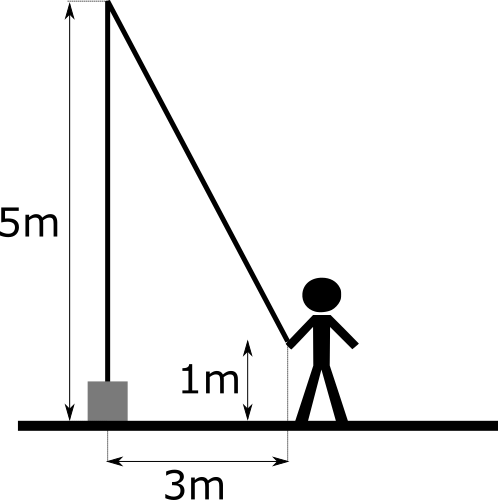
\includegraphics[width=5cm]{pakket.png}
	
	\vspace{3mm}
	
	(A) 0,5 meter \hspace{1cm}
	(B) 0,65 meter \hspace{1cm}
	(C) 0,8 meter \hspace{1cm}
	(D) 0,95 meter
	
%	\vspace{3mm}
%	
%	\begin{numopl}
%		B
%	\end{numopl}
%	

%	\cat{modelleren}
%	\class{**}
%	\opm{manupilatie plaat juni 2014:46\% juist}
%	\info{ijkingstoets juni 2016 - 811 deelnemers} 
%	\juist{62} 
%	\blanco{13} 
%	\ul{upper/lower:85/41\newline percentages ABCD:9/62/11/4}
%\end{oefening}

Deze oefening bekijkt de situatie op 2 momenten.  In realiteit zijn we meestal ge\"interesseerd hoe een toestand evolueert in de tijd.  

\textbf{Opdracht:} 
\begin{enumerate} [(1)]
	\item Schets een grafiek van de hoogte van het pakket als functie van de positie van de man.  Doe dit zonder berekeningen te maken, maar gebruik je intu\"itie.
	\item Wat zorgt voor de beperkingen in het domein en bereik in de functie die je geschetst hebt?
	\item Wat gebeurt er als het touw korter wordt?
\end{enumerate}

Bekijk volgend filmpje en experimenteer met de bijgevoegde applet indien je hier hulp bij nodig hebt.

\vspace{3mm}

\parbox{2cm}{
\includegraphics[width=2cm]{QR_clip_pakket_grafiek.png}}
clip: \href{https://youtu.be/1wCVJ4133o4}{https://youtu.be/1wCVJ4133o4}
\vspace{7mm}

\parbox{2cm}{
\includegraphics[width=2cm]{QR_applet_pakket.png}}
applet: \href{https://www.geogebra.org/m/zyGkhUUE}{https://www.geogebra.org/m/zyGkhUUE}

\vspace{3mm}

Deze oefening illustreert hoe een ingenieur of wetenschapper dikwijls te werk gaat.  Er dient zich een concreet probleem aan, die hij/zij tracht op te lossen door het wiskundig te modelleren.  Tijdens het modelleren en het omzetten naar formules 
gebruikt hij/zij verschillende voorstellingen, waaronder de grafische voorstelling. 
Grafieken zijn een manier om zaken te synthetiseren, om afhankelijkheden tussen parameters te visualiseren.  Werken met grafische voorstellingen laat dikwijls toe om sneller te redeneren, en meer complexe zaken als \'e\'en geheel in je hoofd te hebben.



\newpage

\section{Oefeningen}

\Opensolutionfile{ans}[ans2]

\begin{oefening2}
Bepaal $f\circ g$ en $g\circ f$ met
\[
\begin{array}{lll}
\mbox{a)} & f:x\mapsto \sin(x+2) & g:x\mapsto x+1,\\
\mbox{b)} & f:x\mapsto x+e^x & g:x\mapsto 2x+1,\\
\mbox{c)} & f:x\mapsto x^2 + x & g:x\mapsto e^x + \cos(x^2).
\end{array}
\]

\begin{opl}
\[
\begin{array}{lll}
\mbox{a)} & f\circ g:x\mapsto \sin(x+3) & g\circ f:x\mapsto \sin(x+2)+1\\
\mbox{b)} & f\circ g:x\mapsto 2x+1+e^{2x+1} & g\circ f:x\mapsto 2x+2e^x+1\\
\mbox{c)} & f\circ g:x\mapsto (e^x+\cos(x^2))^2+e^x+\cos(x^2) & g\circ f:x\mapsto
e^{x^2+x}+\cos((x^2+x)^2)
\end{array}
\]
\end{opl}
\end{oefening2}

\begin{oefening2}
Gegeven
\[
\begin{array}{l}
g:x\mapsto x+2,\\
h:x\mapsto 2x,\\
k:x\mapsto 2x-1,
\end{array}
\]
schets voor de functies $f$ hieronder, de grafiek van $f$, $g\circ f$,
$h\circ f$, $k\circ f$, $f \circ g$, $f \circ h$ en $f\circ k$.
\[
\begin{array}{ll}
\mbox{a)} & f:x\mapsto x^2\\
\mbox{b)} & f:x\mapsto x e^{x}\\
\mbox{c)} & f:x\mapsto x+ \sin(x)
\end{array}
\]
\end{oefening2}

\begin{oefening2}
Schets de grafiek van de volgende functies en hun inverse. Bepaal voor
$f$ en $h$ ook het voorschrift van de inverse.
\[
\begin{array}{ll}
\mbox{a)} & f: \R^+ \rightarrow \R: x\mapsto x^2\\
\mbox{b)} & g: \R \rightarrow \R: x\mapsto x + e^x\\
\mbox{c)} & h: [0,4] \rightarrow \R: x\mapsto
 \left\{\ba{ll} 2 x^2 & \mbox{ als } x \in [0,1]\\
               x+1   & \mbox{ als } x \in [1,4]
       \ea\right.
\end{array}
\]
\end{oefening2}

\begin{oefening2}
Schets de grafiek van de volgende functies.
\[
\begin{array}{ll}
\mbox{a)} & x\mapsto x+e^{-x}\\
\mbox{b)} & x\mapsto x-\sin(x)\\
\mbox{c)} & x\mapsto \sin(2x)\\
\mbox{d)} & x\mapsto \sin(2x-1)\\
\mbox{e)} & x\mapsto 3\sin(2x-1)\\
\mbox{f)} & x\mapsto 2(u(x+1)-u(x-1))e^x \mbox{ met $u$ de
  stapfunctie}\\
\mbox{g)} & x\mapsto 1/(1+x^2)\\
\mbox{h)} & x\mapsto \cos(x)/x\\
\mbox{i)} & x\mapsto cos(x)/(1+x^2)\\
\mbox{j)} & x\mapsto e^{-|x|}\\
\mbox{k)} & x\mapsto e^{-x^2}\\
\mbox{l)} & x\mapsto \sin(x^2)\\
\end{array}
\]
\end{oefening2}

\begin{oefening2}
Geef een parametrisatie van\\
\begin{tabular}{ll}
a) & de cirkel met middelpunt $(0,0)$ en straal $2$\\
b) & de cirkel met middelpunt $(1,3)$ en straal $2$\\
c) & de grafiek van $x\mapsto x^2$
\end{tabular}

\begin{opl}
\[
\ba{l}
\mbox{a)~} \phi: [0,2\pi] \rightarrow \R^2: t\mapsto
(2\cos(t),2\sin(t))\\
\mbox{b)~} \phi: [0,2\pi] \rightarrow \R^2: t\mapsto
(1+2\cos(t),3+2\sin(t))\\
\mbox{c~)~} \phi: \R \rightarrow \R^2: t\mapsto
(t,t^2)\\
\mbox{(Andere antwoorden mogelijk!)}
\ea
\]
\end{opl}

\end{oefening2}

\begin{oefening2}
Schets de krommen met volgende parametrisaties
\[
\begin{array}{ll}
\mbox{a)} & \phi: [0,2\pi] \rightarrow \R^2: t\mapsto (2\cos(t),4\sin(t))\\
\mbox{b)} & \phi: [0,2\pi] \rightarrow \R^2: t\mapsto (\sin(t),\cos(t))\\
\mbox{c)} & \phi: \R^+ \rightarrow \R^2: t\mapsto (t^2,t^2)\\
\mbox{d)} & \phi: \R \rightarrow \R^2: t\mapsto (t,t^2)\\
\mbox{e)} & \phi: \R \rightarrow \R^2: t\mapsto (t^2,t)\\
\mbox{f)} & \phi: [0,2\pi] \rightarrow \R^2: t\mapsto (\cos^3(t),\sin^3(t))\\
\end{array}
\]
\end{oefening2}

\newpage
\begin{oefening2}
%\id{modred01**}

Hieronder zie je de grafieken van twee re\"ele functies, links van de functie $f$, rechts van de functie $g$.
De schaal in beide tekeningen is dezelfde. Wat is het verband tussen $g$ en $f$?
\begin{opl}
B
\end{opl}
%\info{februari 2012 - 471 studenten 1e bach W\&T}
%\juist{40}
%\blanco{4}
%\ul{61/15}
%\hfill
%\href{https://videolab.avnet.kuleuven.be/video/?id=626ab0a9a4bfbe8ad8a279d6fd72bd25&height=388&width=640&autostart=false}{\rotatebox{30}{\parbox{3cm}{\includegraphics[height=1cm]{kuleuven.jpg}\\
%\centering{\textcolor{KULblauw}{TipClip}}}}}


\begin{comment}
\psset{unit=0.85cm}
\begin{pspicture}(-3,-0.8)(3,3)
\psaxes[ticks=none,labels=none]{->}(0,0)(-3,-1)(3,3)
\psline(1,0)(1,-0.12)
\rput(1,-0.3){\scriptsize 1}
\psline(0,1)(-0.12,1)
\rput(-0.25,1){\scriptsize 1}
\rput(1,2.5){\small $f$}
\rput(2.8,-0.3){\scriptsize $x$}
\psplot[algebraic,linewidth=1.2pt,plotpoints=300]{-2.9}{2.9}{0.5+(4*x+1.5*cos(5*x-4+x^2/5))/(1+4*x^4)}
\end{pspicture}
\psset{unit=0.8cm}
\begin{pspicture}(-3,-0.8)(3,3)
\psaxes[ticks=none,labels=none]{->}(0,0)(-3,-1)(3,3)
\psline(1,0)(1,-0.12)
\rput(1,-0.3){\scriptsize 1}
\psline(0,1)(-0.12,1)
\rput(-0.25,1){\scriptsize 1}
\rput(1.2,2.5){\small $g$}
\rput(2.8,-0.3){\scriptsize $x$}
\psplot[algebraic,linewidth=1.2pt,plotpoints=300]{-2.9}{2.9}{0.5+(4*(2*x-1)+1.5*cos(5*(2*x-1)-4+(2*x-1)^2/5))/(1+4*(2*x-1)^4)}
\end{pspicture}
\end{comment}

\begin{enumerate}
\item [(A)]Voor alle $x\in\R$ is $g(x)=f(2x+1)$.
\item [(B)] Voor alle $x\in\R$ is $g(x)=f(2x-1)$.
\item [(C)] Voor alle $x\in\R$ is $g(x)=f(x/2+1)$.
\item [(D)] Voor alle $x\in\R$ is $g(x)=f(x/2-1)$.
\item [(E)] Voor alle $x\in\R$ is $g(x)=f(2x-1/2)$.
\end{enumerate}

\bron{Modelvragen ijkingstoets}
\end{oefening2}

\newpage
\begin{oefening2}
%\id{2014red02**}

De grafiek van de re\"ele functie $f$ is gegeven in onderstaande figuur.

\begin{comment}
\psset{unit=1.3cm}
\begin{pspicture}(-0.7,-0.5)(5,2)
\psline{->}(0,0)(4.5,0)
\psline{->}(0,0)(0,1.5)
\psline{-}(1,0)(1,0.1)
\psline{-}(0,1)(0.1,1)
\rput[tl](1,-0.1){1}
\rput[rb](-0.05,1){1}
\rput[rb](-0.05,-0.1){0}
\psplot{0}{1}{x}
\psplot{1}{2}{2 x sub}
\rput[tl](4.55,-0.1){$x$}
\rput[rb](-0.05,1.55){$f(x)$}
\end{pspicture}
\end{comment}

Van de re\"ele functie $g$ weten we dat voor alle $x$ geldt dat $g(x)=f(x^2)$. Welk van onderstaande figuren geeft de grafiek van de functie $g$ weer.


\begin{comment}
\begin{tabbing}

%A
(A)
\begin{pspicture}(-0.7,-0.5)(5,2)
\psline{->}(0,0)(4.5,0)
\psline{->}(0,0)(0,1.5)
\psline{-}(1,0)(1,0.1)
\psline{-}(0,1)(0.1,1)
\rput[tl](1,-0.1){1}
\rput[rb](-0.05,1){1}
\rput[rb](-0.05,-0.1){0}
\psplot{0}{1}{x x mul}
\psplot{1}{4}{x x mul 9 div 8 x mul 9 div sub 16 9 div add}
\rput[tl](4.55,-0.1){$x$}
\rput[rb](-0.05,1.55){$g(x)$}
\end{pspicture}
\hspace {1cm}\=
%B
(B)
\begin{pspicture}(-0.7,-0.5)(5,2)
\psline{->}(0,0)(4.5,0)
\psline{->}(0,0)(0,1.5)
\psline{-}(1,0)(1,0.1)
\psline{-}(0,1)(0.1,1)
\rput[tl](1,-0.1){1}
\rput[rb](-0.05,1){1}
\rput[rb](-0.05,-0.1){0}
\psplot{0}{1}{x x mul}
\psplot{1}{2}{x x mul 4 x mul sub 4 add }
\rput[tl](4.55,-0.1){$x$}
\rput[rb](-0.05,1.55){$g(x)$}

\end{pspicture}
\\
%C
(C)
\begin{pspicture}(-0.7,-0.5)(5,2)
\psline{->}(0,0)(4.5,0)
\psline{->}(0,0)(0,1.5)
\psline{-}(1,0)(1,0.1)
\psline{-}(0,1)(0.1,1)
\rput[tl](1,-0.1){1}
\rput[rb](-0.05,1){1}
\rput[rb](-0.05,-0.1){0}
\psplot{0}{1}{x x mul}
\psplot{1}{1.41}{x x mul 5.828 mul 16.485 x mul sub 11.656 add}
\rput[tl](4.55,-0.1){$x$}
\rput[rb](-0.05,1.55){$g(x)$}

\end{pspicture}
\>
%D
(D)
\begin{pspicture}(-0.7,-0.5)(5,2)
\psline{->}(0,0)(4.5,0)
\psline{->}(0,0)(0,1.5)
\psline{-}(1,0)(1,0.1)
\psline{-}(0,1)(0.1,1)
\rput[tl](1,-0.1){1}
\rput[rb](-0.05,1){1}
\rput[rb](-0.05,-0.1){0}
\psplot{0}{1}{x x mul}
\psplot{1}{4}{16 x x mul sub 15 div }
\rput[tl](4.55,-0.1){$x$}
\rput[rb](-0.05,1.55){$g(x)$}

\end{pspicture}
\\
%E
(E)
\begin{pspicture}(-0.7,-0.5)(5,2)
\psline{->}(0,0)(4.5,0)
\psline{->}(0,0)(0,1.5)
\psline{-}(1,0)(1,0.1)
\psline{-}(0,1)(0.1,1)
\rput[tl](1,-0.1){1}
\rput[rb](-0.05,1){1}
\rput[rb](-0.05,-0.1){0}
\psplot{0}{1}{x x mul}
\psplot{1}{1.41}{2 x x mul sub }
\rput[tl](4.55,-0.1){$x$}
\rput[rb](-0.05,1.55){$g(x)$}

\end{pspicture}

\end{tabbing}
\end{comment}
\begin{opl}
E
\end{opl}

\bron{ijkingstoets september 2014}

\end{oefening2}

\newpage

\begin{oefening2}
%\id{2016red18}

Onderstaande figuur geeft de grafiek van de functie $f:\R\to\R$ weer met een volle lijn en de grafiek van de functie $g:\R \to \R$ met een streepjeslijn.  Welk van onderstaande uitspraken is geldig?

\begin{minipage}{10cm}
   \begin{tikzpicture}[scale=0.5]

        \def\xmin{-10}
        \def\xmax{10}
        \def\ymin{-4}
        \def\ymax{11}
%        \draw[style=help lines, ystep=1, xstep=1] (\xmin,\ymin) grid (\xmax,\ymax);

        \draw (0,0) node[below] {$0$};
				\draw (9,0) node[below] {$x$};
				\draw (0,3) node[left] {$a$};
				\draw (0,6) node[left] {$2a$};
				\draw (0,9) node[left] {$3a$};
				\draw (0,-3) node[left] {$-a$};
				\draw (6,9) node[above] {$f(x)$};
				\draw (6,3) node[above] {$g(x)$};
			
	
				\draw[->]  (-10,0) -- (10,0);
				\draw[->]  (0,-4) -- (0,10);
				\draw[-]  (-0.2,3) -- (0.2,3);
				\draw[-]  (-0.2,6) -- (0.2,6);
			  \draw[-]  (-0.2,9) -- (0.2,9);


        \draw plot [domain=-8:8,samples=300] (\x,{3-6*cos(\x/2 r)});
				\draw[dashed] plot [domain=-8:8] (\x,{-3*cos(\x/2 r)})	;
				

    \end{tikzpicture}
%		\includegraphics[width=8cm]{grafiek.eps}
\end{minipage}
%
\hspace{1cm}
\begin{minipage}{5cm}
\begin{enumerate} 
\item [(A)] $f(x)=g(x)+2a$
\item [(B)] $f(x)=2g(x)+a$
\item [(C)] $f(x)=3g(x)$
\item [(D)] $f(x)=3g(x)+2a$
\end{enumerate}
\end{minipage}

\begin{opl}
B
\end{opl}

%\cat{redeneren}
%\class{*}
%\info{ijkingstoets september 2016 - 206 deelnemers} 
%\juist{61} 
%\blanco{2} 
%\ul{upper/lower:83/38\newline percentages ABCD:0/61/31/5}
%\opm{gebaseerd op vraag 1 sept 2013 met 60\% juist (toen horizontaal geschaald en andere vorm)}
\bron{ijkingstoets september 2016}

\end{oefening2}

\newpage

\section{Oplossing van enkele oefeningen}

\Closesolutionfile{ans}
\begin{Oplossing}{1}
\[
\begin{array}{lll}
\mbox{a)} & f\circ g:x\mapsto \sin(x+3) & g\circ f:x\mapsto \sin(x+2)+1\\
\mbox{b)} & f\circ g:x\mapsto 2x+1+e^{2x+1} & g\circ f:x\mapsto 2x+2e^x+1\\
\mbox{c)} & f\circ g:x\mapsto (e^x+\cos(x^2))^2+e^x+\cos(x^2) & g\circ f:x\mapsto
e^{x^2+x}+\cos((x^2+x)^2)
\end{array}
\]
\end{Oplossing}
\begin{Oplossing}{5}
\[
\ba{l}
\mbox{a)~} \phi: [0,2\pi] \rightarrow \R^2: t\mapsto
(2\cos(t),2\sin(t))\\
\mbox{b)~} \phi: [0,2\pi] \rightarrow \R^2: t\mapsto
(1+2\cos(t),3+2\sin(t))\\
\mbox{c~)~} \phi: \R \rightarrow \R^2: t\mapsto
(t,t^2)\\
\mbox{(Andere antwoorden mogelijk!)}
\ea
\]
\end{Oplossing}
\begin{Oplossing}{7}
B
\end{Oplossing}
\begin{Oplossing}{8}
E
\end{Oplossing}
\begin{Oplossing}{9}
B
\end{Oplossing}


\clearpage{\pagestyle{empty}\cleardoublepage}
\end{document}
